% =========================================================
% Susceptibilidad por movimientos en masa – Cuenca La Iguana
% Regresión Logística y Procesos Gaussianos
% =========================================================
\documentclass[12pt, a4paper]{article}

\usepackage[utf8]{inputenc}
\usepackage[T1]{fontenc}
\usepackage[spanish,es-tabla]{babel}
\usepackage{geometry}
\geometry{margin=2.5cm}
\usepackage{times}
\usepackage{setspace}
\doublespacing

\usepackage{amsmath, amssymb, amsfonts}
\usepackage{graphicx}
\usepackage{subcaption}
\usepackage{float}
\usepackage{booktabs}
\usepackage{array}
\usepackage{tabularx}
\usepackage{multirow}
\usepackage{siunitx}
\usepackage{nicefrac}
\usepackage{xcolor}
\usepackage[colorlinks=true, linkcolor=blue, citecolor=blue, urlcolor=blue]{hyperref}
\usepackage{natbib}
\usepackage{lineno}
\linenumbers

\graphicspath{{FIGURAS/}}

% =========================================================
\begin{document}

% ---- Página de título ----
\begin{titlepage}
\begin{center}

\vspace*{2cm}

{\LARGE\bfseries
Evaluación comparativa de la susceptibilidad por movimientos en masa
en la cuenca La Iguana (Medellín, Colombia) mediante regresión logística
y procesos gaussianos: cuantificación de la incertidumbre
en una cuenca urbana de alta montaña
\par}

\vspace{1.5cm}
{\large Edier Aristizábal$^{1,*}$\par}

\vspace{0.8cm}
{\normalsize
$^1$ Departamento de Geociencias y Medio Ambiente,
Universidad Nacional de Colombia, Medellín, Colombia\\[0.3cm]
$^*$ Correspondencia: evaristizabalg@unal.edu.co
}

\vspace{1.5cm}
{\normalsize
\textit{Manuscrito preparado para envío a}
\textbf{Landslides} -- Springer Nature\\
ISSN 1612-5118
}

\vspace{0.8cm}
{\small \today}

\end{center}

\vspace{1.5cm}
\noindent\textbf{Resumen}

\noindent
Los movimientos en masa constituyen uno de los peligros naturales más recurrentes y devastadores en las regiones montañosas tropicales. En este estudio se presenta un marco probabilístico de dos etapas para la evaluación de la susceptibilidad por movimientos en masa en la cuenca La Iguana (52{,}2 km$^2$, 1465--3141 m s.n.m.), uno de los afluentes del río Medellín con mayor historial de deslizamientos en Colombia. En la primera etapa, un modelo de regresión logística (RL) es ajustado con un conjunto de datos balanceado compuesto por 583 ocurrencias de movimientos en masa y 583 puntos de ausencia seleccionados aleatoriamente, empleando como covariables la pendiente, el aspecto y el Índice Topográfico de Humedad (ITH) derivados de un modelo digital de elevación (MDE) de 10 m de resolución. El modelo RL alcanza un área bajo la curva ROC (AUC) validada con cinco pliegues de $0{,}788 \pm 0{,}025$ y una AUC en el conjunto de prueba de $0{,}778$, confirmando la capacidad discriminativa de los predictores topográficos en este terreno convergente y empinado. En la segunda etapa, un Proceso Gaussiano de Regresión (PGR) con núcleo de Matérn-$\nicefrac{3}{2}$ es condicionado sobre las probabilidades predichas por la RL en las 583 ubicaciones de deslizamientos, produciendo tanto una superficie de susceptibilidad media como un mapa de incertidumbre expresado como desviación estándar posterior en cada celda. El PGR obtiene una AUC de $0{,}765$ sobre la cuadrícula completa de la cuenca y un índice de Brier de $0{,}218$, prácticamente idéntico al de la RL ($0{,}218$), mientras que adicionalmente proporciona intervalos de predicción por celda no disponibles en el enfoque determinístico de la RL. El mapa de incertidumbre del PGR identifica las zonas donde la estimación de susceptibilidad está pobremente restringida, proporcionando una base objetiva para priorizar campañas de validación en campo. Los resultados demuestran que los procesos gaussianos son un complemento práctico e informativo a los métodos estándar de regresión en la cartografía de susceptibilidad por movimientos en masa, y que los atributos topográficos son suficientes para una primera estratificación probabilística del peligro en cuencas andinas complejas.

\vspace{0.5cm}
\noindent\textbf{Palabras clave:} susceptibilidad por movimientos en masa; proceso gaussiano; regresión logística; Índice Topográfico de Humedad; cuantificación de incertidumbre; cuenca La Iguana; Colombia

\end{titlepage}

% =========================================================
\section{Introducción}
\label{sec:introduccion}

Los movimientos en masa —que incluyen deslizamientos traslacionales, flujos de detritos, caídas de roca y avalanchas de tierra— son el peligro natural de mayor recurrencia en las cordilleras tropicales y subtropicales \citep{Varnes1978, Hungr2014}. En Colombia, la confluencia de topografía escarpada, perfiles de meteorización profunda, lluvia convectiva intensa y expansión urbana acelerada crea condiciones de riesgo persistentemente elevadas \citep{Aristizabal2023}. El Área Metropolitana del Valle de Aburrá, centrada en Medellín, ha registrado centenares de eventos fatales durante las últimas cuatro décadas, siendo las subcuencas de la vertiente occidental de la Cordillera Central las más afectadas \citep{Salazar2018}.

La cartografía de susceptibilidad por movimientos en masa (CSMM) estima la probabilidad espacial de falla, constituyendo el fundamento para la zonificación del riesgo, la planificación territorial, los sistemas de alerta temprana y el diseño de infraestructura \citep{Guzzetti2005, Corominas2014}. Durante los últimos treinta años se ha desarrollado un amplio espectro de enfoques estadísticos y de aprendizaje automático para la CSMM, desde métodos bivariados hasta regresión logística (RL), máquinas de soporte vectorial, bosques aleatorios y redes neuronales profundas \citep{Reichenbach2018}. Entre estos, la RL sigue siendo el método más ampliamente adoptado por su interpretabilidad estadística, estructura de coeficientes transparente y protocolos de validación bien establecidos \citep{Atkinson1998, Budimir2015, Lombardo2018}. Sin embargo, la RL produce una estimación puntual de la probabilidad sin intervalos de incertidumbre explícitos sobre la superficie predicha, lo que dificulta la comunicación del riesgo y la identificación de zonas donde se requiere recolección adicional de datos.

Los procesos gaussianos (PG) ofrecen una alternativa bayesiana no paramétrica que modela no solo la susceptibilidad esperada sino también la incertidumbre de esa estimación en cada ubicación \citep{Rasmussen2006}. El prior del PG codifica creencias a priori sobre la suavidad de la función a través de un núcleo de covarianza cuyos hiperparámetros son optimizados maximizando la verosimilitud marginal logarítmica, evitando elecciones arbitrarias de regularización. Aplicaciones previas de PG a georriesgos incluyen la predicción del movimiento del suelo sísmico \citep{Lombardo2020} y el modelado por proceso de puntos de flujos de detritos \citep{Lombardo2019}, pero su uso en la CSMM basada en atributos del terreno es aún escaso.

En este artículo se propone y evalúa un marco de dos etapas: (i) un modelo de regresión logística entrenado sobre un conjunto de datos balanceado de presencias y ausencias para producir una superficie de susceptibilidad probabilística sobre la cuadrícula completa de 10 m, y (ii) un Proceso Gaussiano de Regresión (PGR) condicionado sobre las probabilidades predichas por la RL en las ubicaciones de deslizamientos conocidos, generando tanto una media posterior como una desviación estándar posterior para cada celda del MDE. Se aplica este marco a la cuenca La Iguana, un afluente de 52{,}2 km$^2$ en Medellín para el que se dispone de un inventario completo de movimientos en masa derivado de levantamientos multifuente. Los objetivos específicos son:

\begin{enumerate}
    \item Cuantificar el desempeño discriminativo de la RL con covariables topográficas (pendiente, aspecto, ITH) en una cuenca urbana andina de alta pendiente;
    \item Desarrollar un modelo de PG que reproduzca la señal de la RL en las ubicaciones de deslizamientos y la extrapole probabilísticamente al espacio de covariables completo;
    \item Generar mapas de incertidumbre celda por celda que revelen dónde la estimación de susceptibilidad es menos confiable;
    \item Comparar ambos modelos mediante métricas múltiples de desempeño y distribuciones de clases de susceptibilidad.
\end{enumerate}

Los resultados contribuyen a la creciente literatura que aboga por la cartografía de susceptibilidad consciente de la incertidumbre como prerequisito para políticas de gestión del riesgo basadas en evidencia.

% =========================================================
\section{Área de estudio}
\label{sec:area}

La cuenca La Iguana (Fig.~\ref{fig:covariables}) está ubicada en la vertiente occidental de la Cordillera Central dentro del Valle de Aburrá, drenando aproximadamente 52{,}2 km$^2$ de terreno montañoso empinado hacia el río Medellín. La cuenca ocupa una posición central dentro del área metropolitana y ha sido escenario de numerosos movimientos en masa documentados, incluyendo deslizamientos traslacionales superficiales, flujos de detritos y fallas profundas complejas.

\subsection{Topografía y geología}

Las elevaciones dentro de la cuenca oscilan entre aproximadamente 1465 m y 3141 m s.n.m., con una elevación media cercana a los 2100 m y un relieve fuertemente disectado creado por la red de drenaje orientada NNO. Las pendientes son generalmente escarpadas (media $\approx 30°$, localmente superando los $70°$) y el terreno exhibe las concavidades convergentes típicas de cuencas coluviales dominadas por cárcavas y regueros \citep{Salazar2018}. El substrato geológico está compuesto predominantemente por esquistos y gneis metamórficos del Complejo Cajamarca, localmente intruidos por monzonitas de cuarzo, todos intensamente meteorizados hasta formar perfiles de saprolito de 5 a 20 m de profundidad. Depósitos coluviales y aluviales se presentan a lo largo del fondo del valle y las laderas inferiores.

\subsection{Clima e hidrología}

La cuenca tiene un clima tropical bimodal controlado por la oscilación latitudinal de la Zona de Convergencia Intertropical (ZCIT), con temporadas lluviosas en abril-mayo y septiembre-noviembre, y períodos más secos en diciembre-febrero y junio-agosto. La precipitación media anual varía de aproximadamente 1800 mm en el fondo del valle a más de 3000 mm cerca de la divisoria de aguas. Las tormentas convectivas de corta duración (1 a 6 h) e intensidad elevada (frecuentemente superando los 50 mm h$^{-1}$) son el mecanismo primario de desencadenamiento de movimientos en masa en este entorno \citep{Aristizabal2023}.

\subsection{Historial de movimientos en masa}

El inventario de movimientos en masa empleado en este estudio hace parte del catálogo regional del Valle de Aburrá, compilado mediante interpretación sistemática de imágenes de teledetección, registros históricos y levantamientos de campo. Un total de 5689 eventos de movimientos en masa georreferenciados están documentados para el área metropolitana; de estos, 583 se localizan dentro de la cuenca La Iguana. El inventario incluye deslizamientos traslacionales superficiales, caídas de roca, flujos de detritos y flujos de tierra, sin distinción de tipo en el modelado de susceptibilidad, siguiendo la práctica común de agrupar tipos de falla cuando la resolución de los datos no permite discriminación.

% =========================================================
\section{Datos y metodología}
\label{sec:metodos}

\subsection{Modelo Digital de Elevación y preprocesamiento}

Se utilizó un MDE de 10 m de resolución, derivado de levantamientos LiDAR y restitución fotogramétrica en el sistema de coordenadas proyectado MAGNA-SIRGAS 2018 / Origen Nacional. El MDE fue recortado al límite de la cuenca La Iguana, obteniendo un dominio de análisis válido de 521{,}586 celdas. Previo a la derivación de atributos del terreno, se aplicó un acondicionamiento hidrológico: relleno de depresiones, eliminación de zonas planas y resolución de ambigüedades de dirección de flujo, utilizando la biblioteca \texttt{pysheds}.

\subsection{Derivación de atributos del terreno}

Se derivaron tres atributos topográficos como covariables en ambos modelos (Fig.~\ref{fig:covariables}):

\subsubsection{Pendiente}

La pendiente ($\beta$, en grados) cuantifica el gradiente local del terreno y es el principal motor de la desestabilización gravitacional. Se calculó mediante diferencias finitas centrales del MDE:

\begin{equation}
    \beta = \arctan\!\left(\sqrt{\left(\frac{\partial z}{\partial x}\right)^2 + \left(\frac{\partial z}{\partial y}\right)^2}\right)
    \label{eq:pendiente}
\end{equation}

\noindent donde $z$ es la elevación y $x$, $y$ son las coordenadas espaciales. Los valores de pendiente dentro de la cuenca oscilan entre $0°$ y $89{,}2°$, con fuerte concentración entre $20°$ y $45°$ en los flancos principales del valle.

\subsubsection{Aspecto}

El aspecto ($\alpha$, en grados desde el norte, medido en sentido horario) refleja la dirección del descenso más pronunciado y sirve como proxy de la carga de radiación solar, la asimetría de humedad del suelo y la exposición de la vegetación, todos los cuales modulan la meteorización y la cohesión radicular:

\begin{equation}
    \alpha = \left[\arctan\!\left(\frac{-\partial z/\partial x}{\partial z/\partial y}\right)\right] \bmod 360°
    \label{eq:aspecto}
\end{equation}

\subsubsection{Índice Topográfico de Humedad}

El Índice Topográfico de Humedad \citep[ITH;][]{BandaKirkby1979} es un proxy en estado estacionario de la tendencia de una celda a acumular agua en el suelo:

\begin{equation}
    \mathrm{ITH} = \ln\!\left(\frac{a}{\tan\beta}\right)
    \label{eq:ith}
\end{equation}

\noindent donde $a$ (m) es el área específica de contribución aguas arriba —el área de drenaje aguas arriba por unidad de longitud de contorno— calculada mediante el algoritmo de flujo de dirección única D8 \citep{OCallaghan1984}. Valores elevados del ITH indican posiciones topográficas convergentes (hondonadas, fondos de valle) propensas a la saturación transitoria y al aumento de la presión de poros. Dentro de la cuenca La Iguana, el ITH varía de $-1{,}2$ a $20{,}2$, con valores superiores a 12 concentrados a lo largo de la red de drenaje principal.

\subsection{Diseño de muestreo}

Se adoptó una estrategia de muestreo balanceado de presencias y ausencias. Los 583 eventos de movimientos en masa definen el conjunto de presencias. Un número igual de puntos de ausencia (fondo) fue seleccionado mediante muestreo aleatorio simple de las celdas válidas dentro de la cuenca, excluyendo cualquier celda ocupada por un deslizamiento conocido. Los valores de las covariables en cada punto de muestreo fueron extraídos de las celdas ráster correspondientes mediante remuestreo al vecino más cercano usando la transformación afín del MDE.

Esta proporción 1:1 presencia-ausencia sigue la recomendación de \citet{Heckmann2014} para modelos de susceptibilidad basados en regresión logística y produce una probabilidad de clase a priori no informativa ($\pi = 0{,}5$), de modo que los coeficientes del modelo reflejan la discriminación genuina de las covariables en lugar del desequilibrio de etiquetas. El conjunto de datos combinado ($n = 1166$) fue dividido 70:30 en subconjuntos de entrenamiento y prueba mediante muestreo aleatorio estratificado para preservar la proporción de clases.

\subsection{Regresión logística}
\label{sec:rl}

La regresión logística modela la probabilidad condicional de ocurrencia de un movimiento en masa como:

\begin{equation}
    P(Y = 1 \mid \mathbf{x}) = \sigma\!\left(\beta_0 + \boldsymbol{\beta}^\top \mathbf{x}\right) = \frac{1}{1 + \exp\!\left(-(\beta_0 + \boldsymbol{\beta}^\top \mathbf{x})\right)}
    \label{eq:rl}
\end{equation}

\noindent donde $\mathbf{x} = (\text{pendiente},\, \text{aspecto},\, \text{ITH})^\top$ es el vector de covariables estandarizado y $\sigma(\cdot)$ es la función sigmoide logística. La log-verosimilitud se maximiza sujeta a una penalización de regularización $\ell_2$ con fortaleza $C = 1{,}0$ (equivalente a $\lambda = 1/C$ en la convención $-\log\mathcal{L} + \lambda\|\boldsymbol{\beta}\|^2$), implementada mediante el optimizador L-BFGS-B.

Todas las covariables fueron estandarizadas (media cero, varianza unitaria) antes del ajuste del modelo para garantizar que las magnitudes de los coeficientes sean directamente comparables y para evitar mal condicionamiento en la optimización. Los coeficientes ajustados se interpretan como el cambio en el log-momio de ocurrencia de movimientos en masa por un incremento de una desviación estándar en cada predictor.

El desempeño del modelo fue evaluado mediante validación cruzada estratificada de cinco pliegues con la AUC-ROC como criterio de puntuación, complementada con métricas en el conjunto de prueba separado: AUC, Precisión Promedio (AP), exactitud, precisión, exhaustividad, puntuación F1 y el índice de Brier \citep{Brier1950, Fawcett2006}.

El modelo RL calibrado fue aplicado a las 521{,}586 celdas válidas de la cuenca para producir un ráster de susceptibilidad probabilística completo.

\subsection{Proceso Gaussiano de Regresión}
\label{sec:pg}

\subsubsection{Formulación del modelo}

Un proceso gaussiano es una distribución sobre funciones $f: \mathbb{R}^d \to \mathbb{R}$ completamente especificada por una función media $m(\mathbf{x})$ y una función de covarianza (núcleo) $k(\mathbf{x}, \mathbf{x}')$ \citep{Rasmussen2006}:

\begin{equation}
    f(\mathbf{x}) \sim \mathcal{GP}\!\left(m(\mathbf{x}),\; k(\mathbf{x}, \mathbf{x}')\right)
    \label{eq:pg_prior}
\end{equation}

Se utilizan como objetivos de entrenamiento los valores normalizados $\tilde{y}_i = \hat{p}_\mathrm{RL}(\mathbf{x}_i)$ —las probabilidades predichas por la RL en las $n_{DS} = 580$ celdas únicas de deslizamientos (tras eliminar colisiones de celdas duplicadas)—. El PG aprende entonces el mapeo $\mathbf{x} \mapsto \hat{p}_\mathrm{RL}(\mathbf{x})$ y, fundamentalmente, proporciona una distribución posterior sobre este mapeo en lugar de una predicción puntual. El PG es ajustado en el espacio de covariables estandarizado.

Dado el conjunto de entrenamiento $\mathcal{D} = \{(\mathbf{x}_i, \tilde{y}_i)\}_{i=1}^{n}$ con ruido gaussiano asumido $\varepsilon \sim \mathcal{N}(0, \sigma_n^2)$, la distribución predictiva posterior en un nuevo punto $\mathbf{x}_*$ es:

\begin{align}
    \mu(\mathbf{x}_*) &= \mathbf{k}_*^\top \left(\mathbf{K} + \sigma_n^2 \mathbf{I}\right)^{-1} \tilde{\mathbf{y}} \label{eq:pg_media}\\
    \sigma^2(\mathbf{x}_*) &= k(\mathbf{x}_*, \mathbf{x}_*) - \mathbf{k}_*^\top \left(\mathbf{K} + \sigma_n^2 \mathbf{I}\right)^{-1} \mathbf{k}_* \label{eq:pg_var}
\end{align}

\noindent donde $\mathbf{K}_{ij} = k(\mathbf{x}_i, \mathbf{x}_j)$ es la matriz de Gram $n \times n$ del conjunto de entrenamiento y $\mathbf{k}_*$ es el vector $n$-dimensional de covarianzas entre el punto de prueba y todos los puntos de entrenamiento. La media posterior $\mu(\mathbf{x}_*)$ es la predicción de susceptibilidad del PG y $\sigma(\mathbf{x}_*)$ es la incertidumbre asociada (desviación estándar).

\subsubsection{Núcleo de covarianza}

Se empleó un núcleo compuesto que combina un término de amplitud de señal, una función de covarianza de Matérn-$\nicefrac{3}{2}$ \citep{Matern1960} y un nugget de ruido blanco:

\begin{equation}
    k(\mathbf{x}, \mathbf{x}') = \sigma_f^2 \left(1 + \frac{\sqrt{3}\,r}{l}\right)\exp\!\left(-\frac{\sqrt{3}\,r}{l}\right) + \sigma_n^2\,\delta(\mathbf{x}, \mathbf{x}')
    \label{eq:nucleo}
\end{equation}

\noindent donde $r = \|\mathbf{x} - \mathbf{x}'\|$ es la distancia euclidiana en el espacio de covariables estandarizado, $\sigma_f^2$ es la varianza de la señal, $l$ es la longitud de escala y $\sigma_n^2$ es la varianza del ruido. El núcleo de Matérn-$\nicefrac{3}{2}$ fue preferido sobre el exponencial cuadrático (función de base radial) porque genera funciones muestrales exactamente una vez diferenciables, lo que es más consistente con la expectativa física de cambios abruptos pero no discontinuos en la susceptibilidad impulsada por el terreno.

Los tres hiperparámetros $(\sigma_f, l, \sigma_n)$ fueron optimizados maximizando la log-verosimilitud marginal con cinco reinicios aleatorios para mitigar óptimos locales. El núcleo optimizado arrojó $\hat{\sigma}_f = 0{,}924$, $\hat{l} = 10{,}0$ (en unidades de covariables estandarizadas) y $\hat{\sigma}_n = 0{,}010$, indicando una señal fuerte y suave con contribución mínima del nugget.

\subsubsection{Consideraciones computacionales}

La inferencia estándar en PG requiere operaciones $\mathcal{O}(n^3)$ para la descomposición de Cholesky de la matriz de Gram y $\mathcal{O}(n^2)$ de memoria, lo que es prohibitivo para el conjunto completo de 580 puntos de entrenamiento. Por tanto, se aplicó un submuestreo aleatorio a 400 puntos previo al ajuste del PG. La predicción sobre las 521{,}586 celdas de la cuenca se realizó en minilotes de 5000 celdas para mantener el uso de memoria acotado.

El PG fue implementado usando la clase \texttt{GaussianProcessRegressor} de \texttt{scikit-learn} \citep{Pedregosa2011} con la opción \texttt{normalize\_y=True}, que normaliza internamente los objetivos a media cero y varianza unitaria antes del ajuste y retrotransforma las predicciones y las incertidumbres.

\subsection{Evaluación y clasificación de la susceptibilidad}

Ambos modelos fueron evaluados sobre la cuadrícula completa de la cuenca ($n = 521{,}586$ celdas) frente al mapa binario de ocurrencia de movimientos en masa (1 = celda con deslizamiento, 0 = todas las demás celdas válidas), reconociendo el fuerte desequilibrio de clases natural ($583/521{,}586 \approx 0{,}11\%$). Se calcularon las siguientes métricas:

\begin{itemize}
    \item \textbf{AUC-ROC}: Área bajo la curva ROC —métrica de discriminación independiente del umbral \citep{Fawcett2006}—;
    \item \textbf{Precisión Promedio (AP)}: Área bajo la curva Precisión-Exhaustividad, más informativa bajo desequilibrio severo de clases que la AUC-ROC;
    \item \textbf{Índice de Brier}: $\mathrm{IB} = n^{-1}\sum_{i=1}^{n}(\hat{p}_i - y_i)^2$, regla de puntuación propia que mide conjuntamente la calibración y la agudeza \citep{Brier1950};
    \item \textbf{Exactitud, precisión, exhaustividad, F1}: Métricas de clasificación dependientes del umbral calculadas en el límite de decisión $\hat{p} = 0{,}5$.
\end{itemize}

La susceptibilidad fue clasificada en cinco clases cualitativas usando intervalos de probabilidad iguales: Muy Baja ($<0{,}2$), Baja ($0{,}2$--$0{,}4$), Moderada ($0{,}4$--$0{,}6$), Alta ($0{,}6$--$0{,}8$) y Muy Alta ($>0{,}8$). Se calculó la proporción del área de la cuenca en cada clase para el modelo RL.

Todo el análisis fue realizado en Python 3.13 usando \texttt{NumPy}, \texttt{Pandas}, \texttt{GeoPandas}, \texttt{Rasterio}, \texttt{pysheds} y \texttt{scikit-learn} \citep{Pedregosa2011}. El análisis reproducible completo está disponible como cuaderno Jupyter en el material suplementario.

% =========================================================
\section{Resultados}
\label{sec:resultados}

\subsection{Covariables del terreno}

Los tres atributos del terreno derivados exhiben patrones espaciales contrastantes dentro de la cuenca (Fig.~\ref{fig:covariables}). La pendiente es más elevada a lo largo de las incisiones del canal principal y las crestas secundarias (55--70°), y disminuye hacia las mesetas superiores y los fondos de valle. La distribución del ITH refleja la red de drenaje altamente dendrítica, con valores superiores a 14 concentrados en hondonadas convergentes y márgenes del canal —zonas donde la humedad antecedente del suelo y las presiones de poros transitorias tienen mayor probabilidad de alcanzar los umbrales de falla durante eventos de lluvia intensa—. El aspecto es espacialmente diverso, aunque se observa una ligera asimetría entre las laderas orientadas al N-NO (más húmedas, más vegetadas) y las expuestas al S-SE.

\begin{figure}[H]
    \centering
    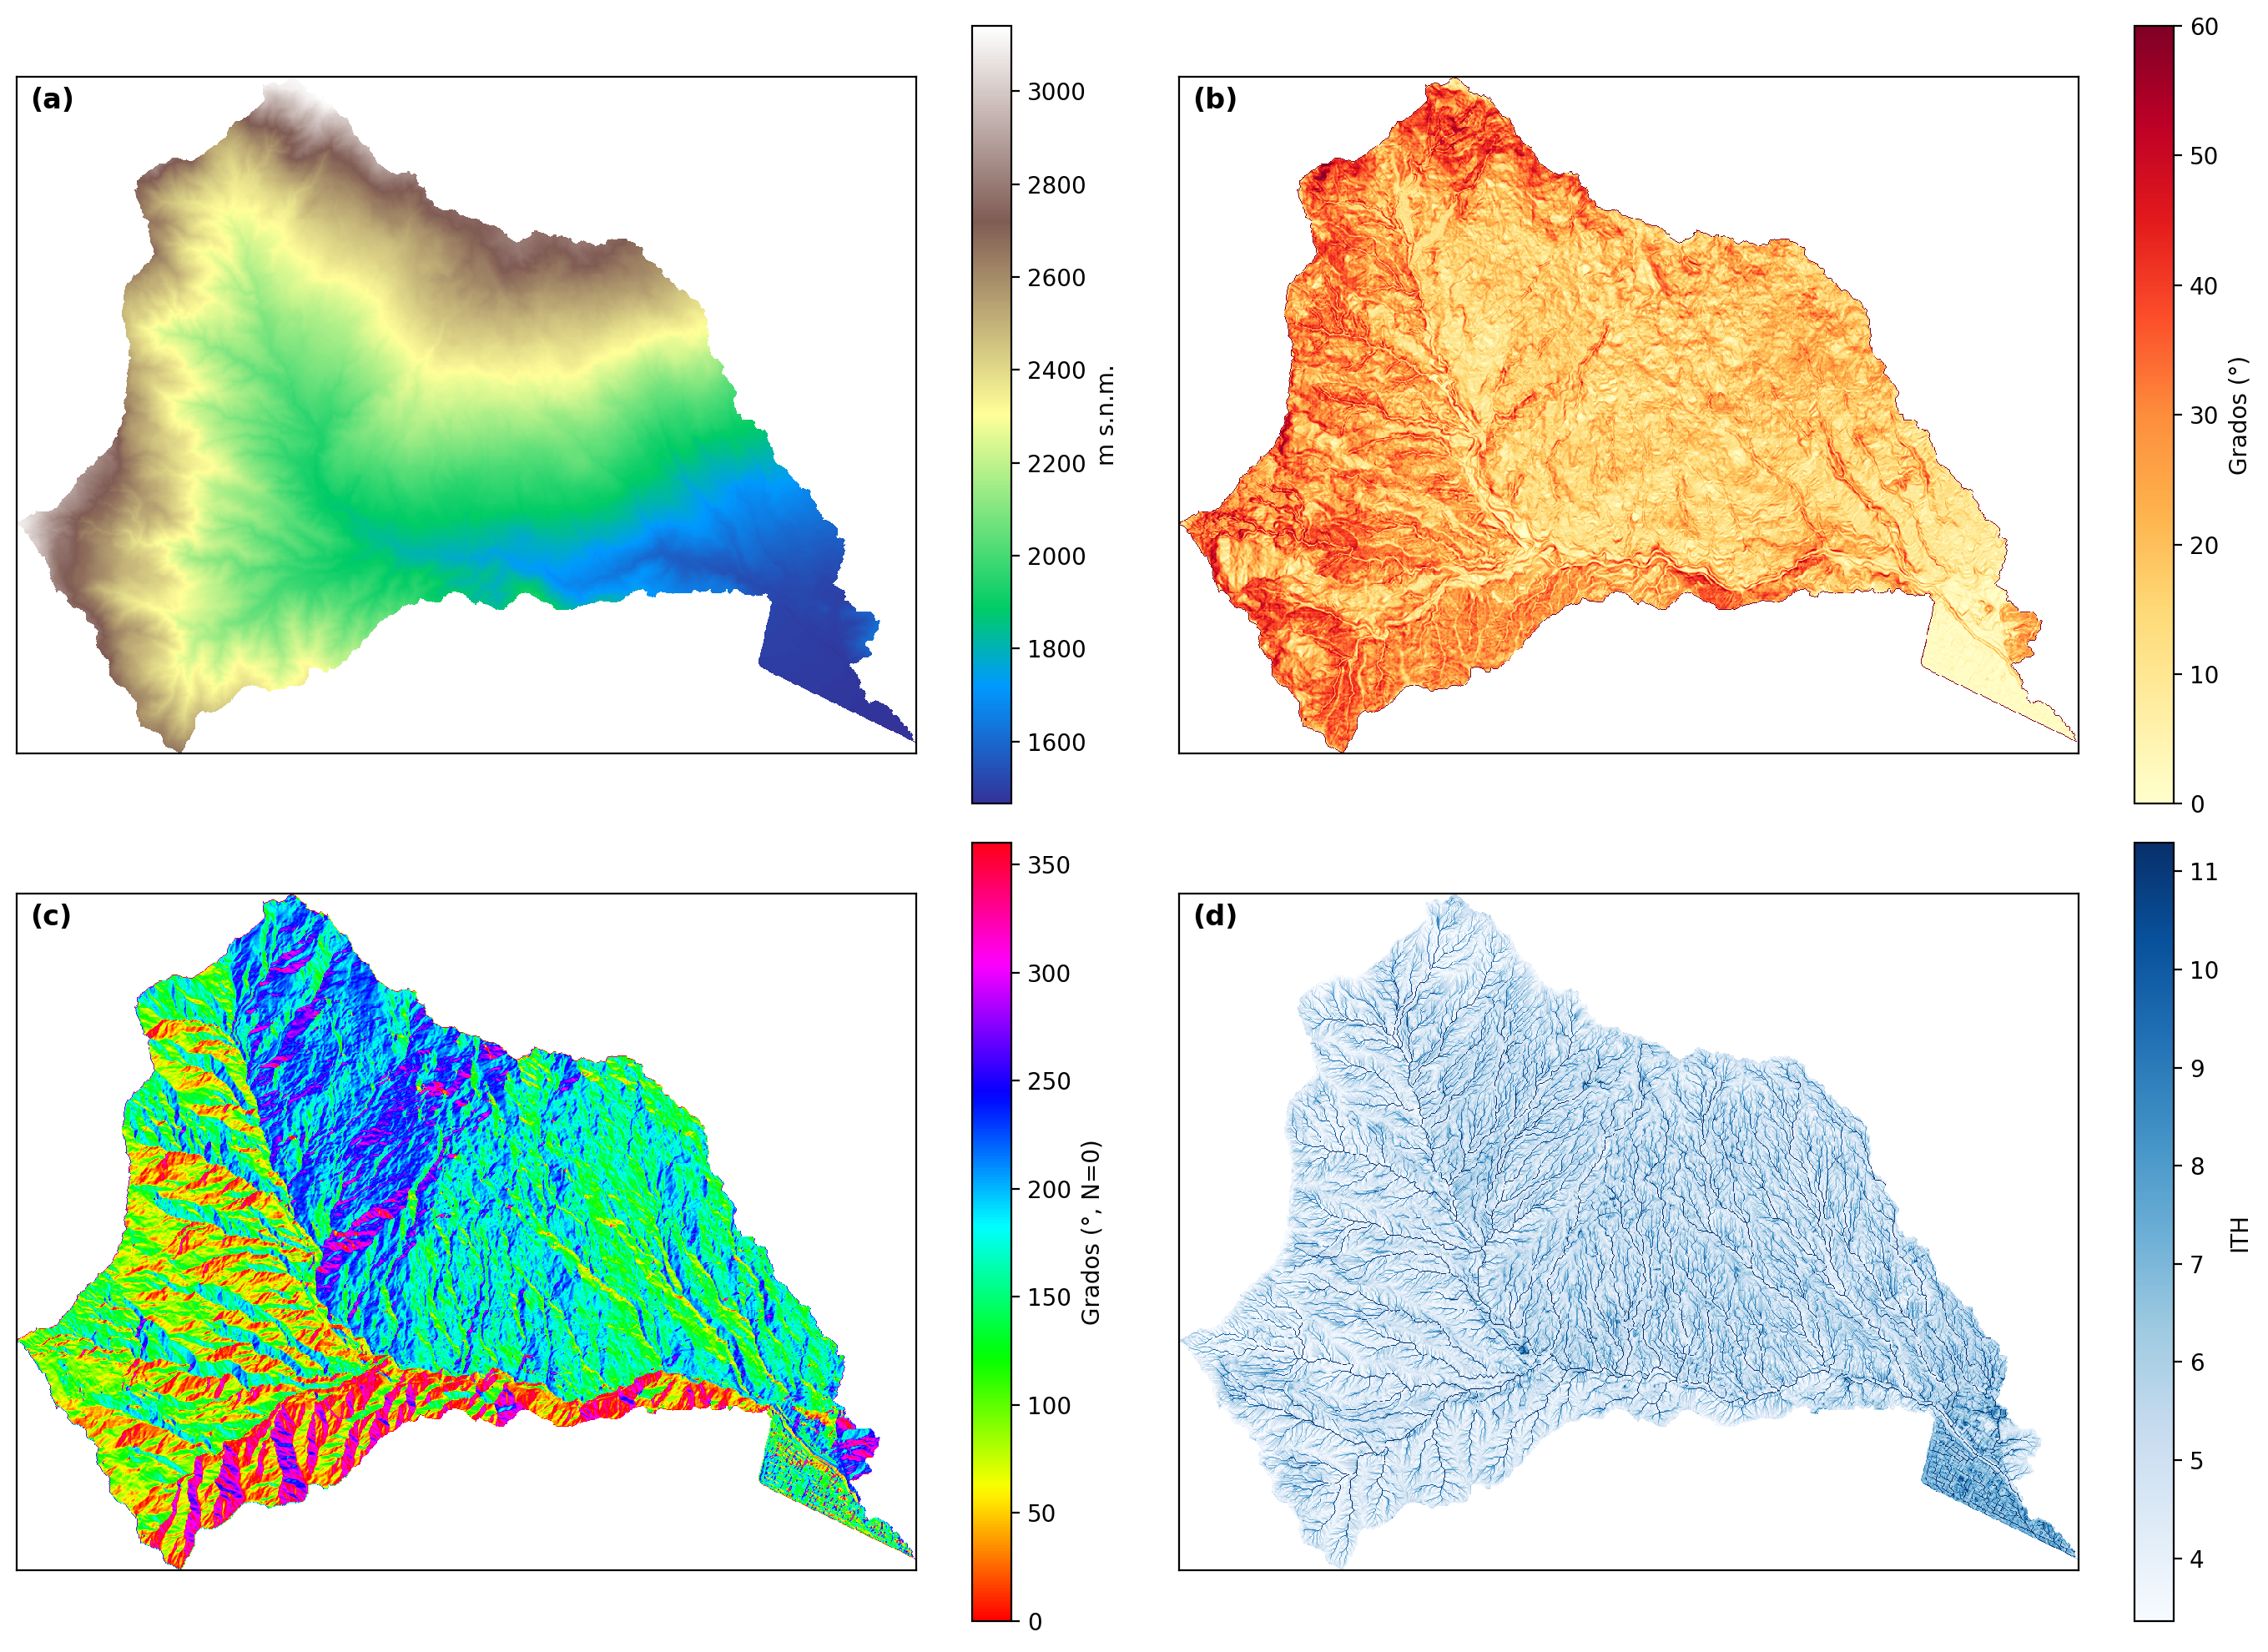
\includegraphics[width=\textwidth]{Fig1_terrain_covariates.png}
    \caption{Covariables del terreno derivadas del MDE de 10 m para la cuenca La Iguana: (a) elevación (m s.n.m.), (b) pendiente (grados), (c) aspecto (grados desde el norte en sentido horario) e (d) Índice Topográfico de Humedad (ITH). Todas las capas están recortadas al límite de la cuenca.}
    \label{fig:covariables}
\end{figure}

\subsection{Distribuciones de covariables en ubicaciones de deslizamientos y fondo}

La Figura~\ref{fig:distribuciones} muestra las densidades de probabilidad empíricas de cada covariable en los sitios de deslizamientos y en los puntos de fondo. Los sitios de deslizamiento presentan un desplazamiento marcado hacia pendientes más pronunciadas (mediana $\approx 35°$ frente a $\approx 28°$ para el fondo), consistente con la reconocida asociación positiva entre el gradiente de pendiente y la probabilidad de falla. La distribución del aspecto en las ubicaciones de deslizamientos muestra una ligera concentración en el cuadrante NO ($270°$--$360°$) respecto al fondo, posiblemente reflejando microclimas más húmedos y meteorización más profunda en laderas menos expuestas al sol. Las distribuciones del ITH no muestran una separación bimodal fuerte, lo que sugiere que a 10 m de resolución la señal hidrológica directa queda parcialmente enmascarada por el promediado espacial de las áreas de contribución.

\begin{figure}[H]
    \centering
    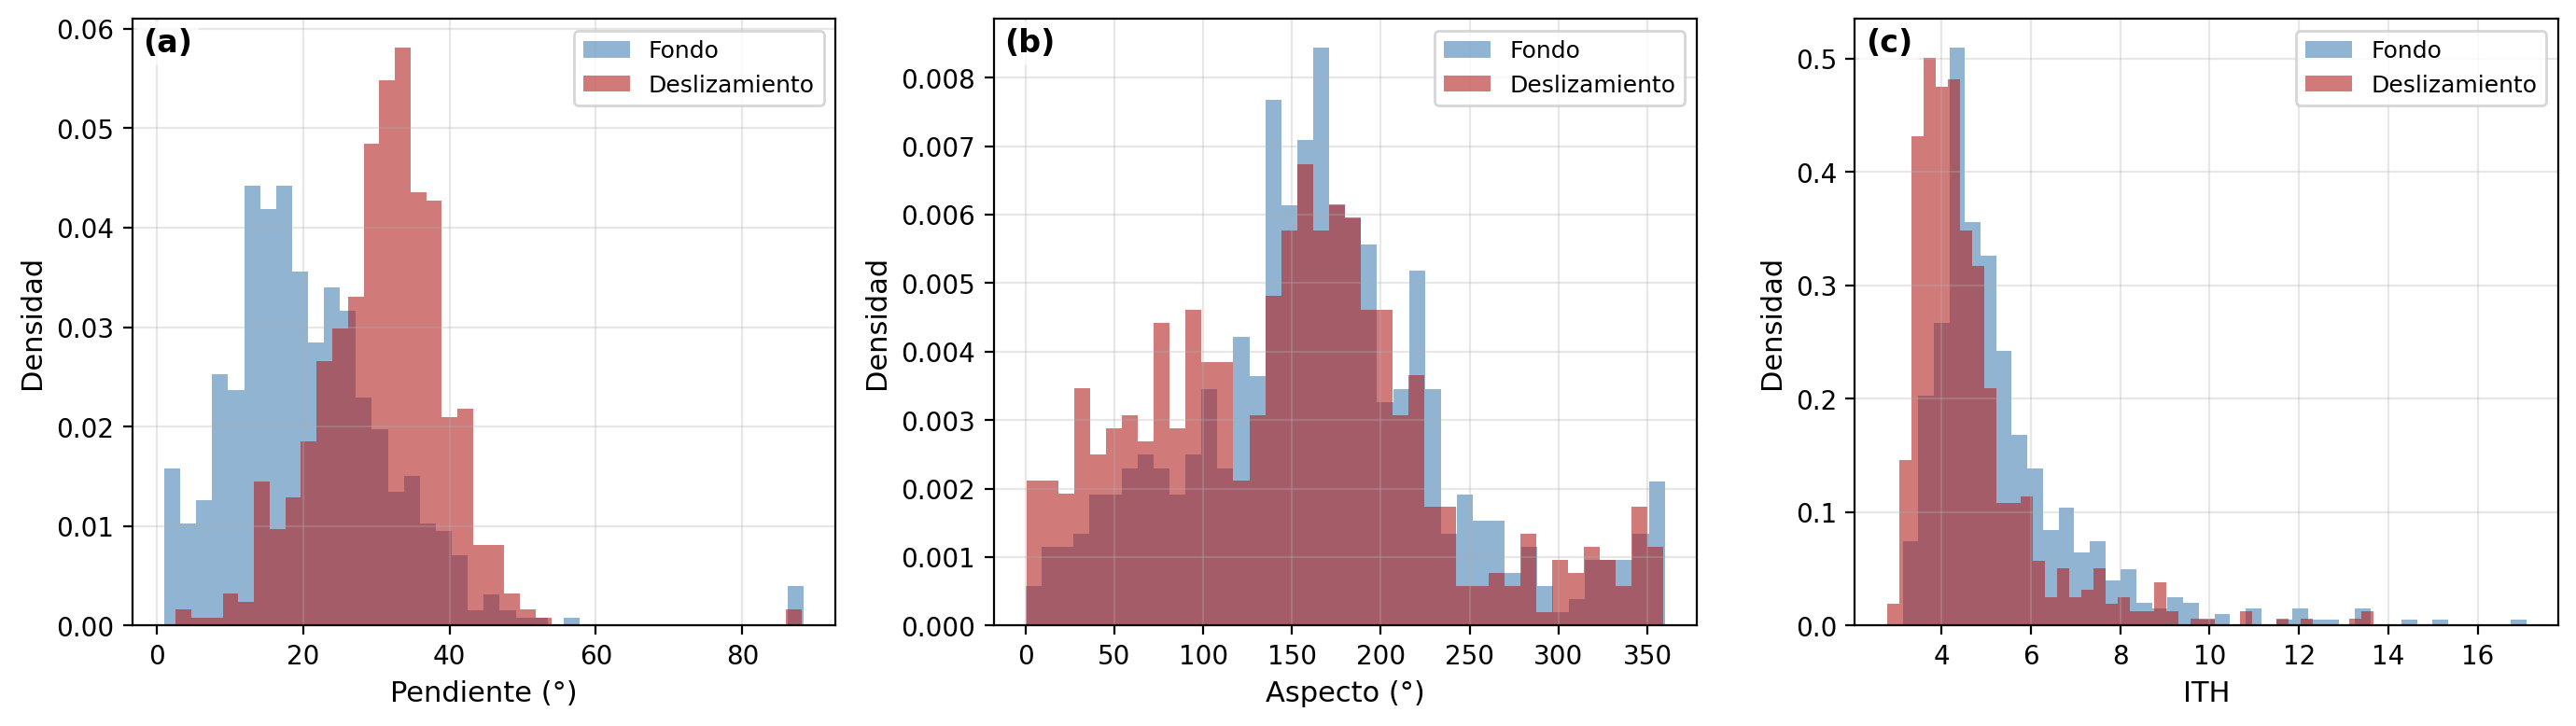
\includegraphics[width=\textwidth]{Fig6_covariate_distributions.png}
    \caption{Distribuciones de densidad de probabilidad empírica de las covariables del terreno en ubicaciones de deslizamientos (rojo) y en puntos de fondo (azul): (a) pendiente, (b) aspecto e (c) Índice Topográfico de Humedad. Estimaciones de densidad basadas en $n = 583$ puntos por clase.}
    \label{fig:distribuciones}
\end{figure}

\subsection{Modelo de regresión logística}

El modelo RL ajustado alcanza una AUC de prueba de $0{,}778$ y una AUC validada con cinco pliegues de $0{,}788 \pm 0{,}025$, indicando buena discriminación y generalización estable en la extensión espacial de la cuenca (Tabla~\ref{tab:metricas}). Las curvas ROC y de Precisión-Exhaustividad se muestran en la Figura~\ref{fig:evaluacion}. Los coeficientes de regresión estandarizados (Tabla~\ref{tab:coeficientes}) confirman que la pendiente es el predictor dominante ($\hat{\beta}_\mathrm{pendiente} = +1{,}193$), incrementando el log-momio de ocurrencia de movimientos en masa en 1,19 por incremento de una desviación estándar en la pendiente. El aspecto tiene una influencia negativa débil ($\hat{\beta}_\mathrm{aspecto} = -0{,}103$), indicando ligeramente mayor susceptibilidad en laderas orientadas al norte controlando por el gradiente de pendiente. El ITH tiene un coeficiente estandarizado casi nulo ($\hat{\beta}_\mathrm{ITH} = -0{,}011$), sugiriendo que a 10 m de resolución el proxy hidrológico en estado estacionario no añade poder discriminativo sustancial más allá del capturado por la pendiente.

\begin{table}[H]
    \centering
    \caption{Coeficientes estandarizados de la regresión logística e intercepto.}
    \label{tab:coeficientes}
    \begin{tabular}{lccc}
        \toprule
        Predictor & Coeficiente ($\hat{\beta}$) & Momio relativo (e$^{\hat{\beta}}$) \\
        \midrule
        Pendiente  & $+1{,}193$ & 3{,}30 \\
        Aspecto    & $-0{,}103$ & 0{,}90 \\
        ITH        & $-0{,}011$ & 0{,}99 \\
        Intercepto & $-0{,}007$ & --    \\
        \bottomrule
    \end{tabular}
\end{table}

\begin{figure}[H]
    \centering
    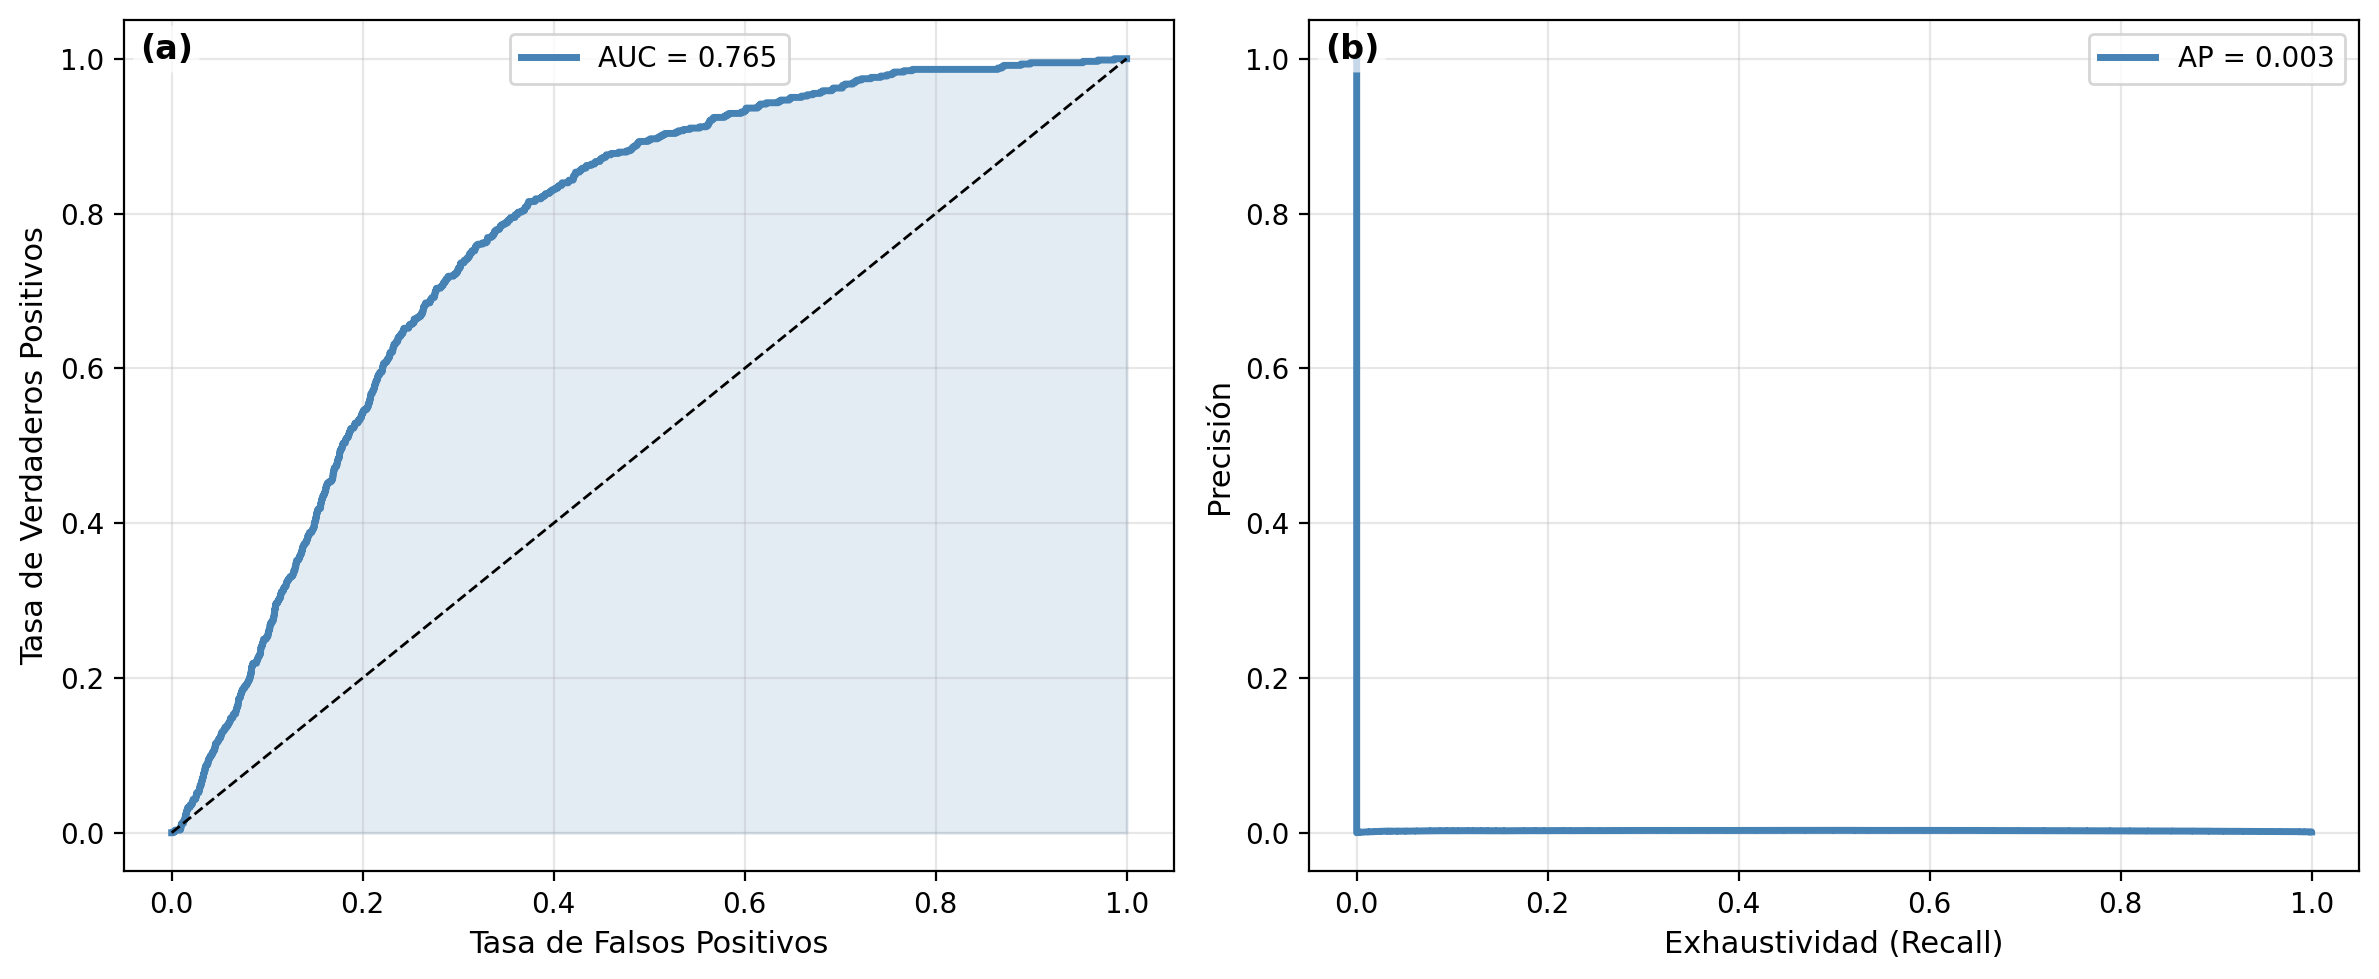
\includegraphics[width=\textwidth]{Fig2_model_evaluation.png}
    \caption{Evaluación del modelo de regresión logística aplicado a la cuadrícula completa de la cuenca La Iguana: (a) curva ROC con el área bajo la curva (AUC = 0,765) y (b) curva Precisión-Exhaustividad con la Precisión Promedio (AP = 0,003). El área sombreada representa la superficie bajo cada curva.}
    \label{fig:evaluacion}
\end{figure}

El mapa de susceptibilidad RL (Fig.~\ref{fig:mapa_rl}) muestra una fuerte asociación espacial entre probabilidades elevadas ($P > 0{,}6$) y las laderas coluviales empinadas que flanquean el canal principal y sus afluentes, particularmente entre 1700 y 2400 m. Las zonas más planas cerca de la divisoria de aguas y el fondo del valle exhiben probabilidades predichas bajas. Los 583 puntos de deslizamientos mapeados se superponen predominantemente sobre zonas de alta susceptibilidad, cualitativamente consistente con la AUC positiva.

\begin{figure}[H]
    \centering
    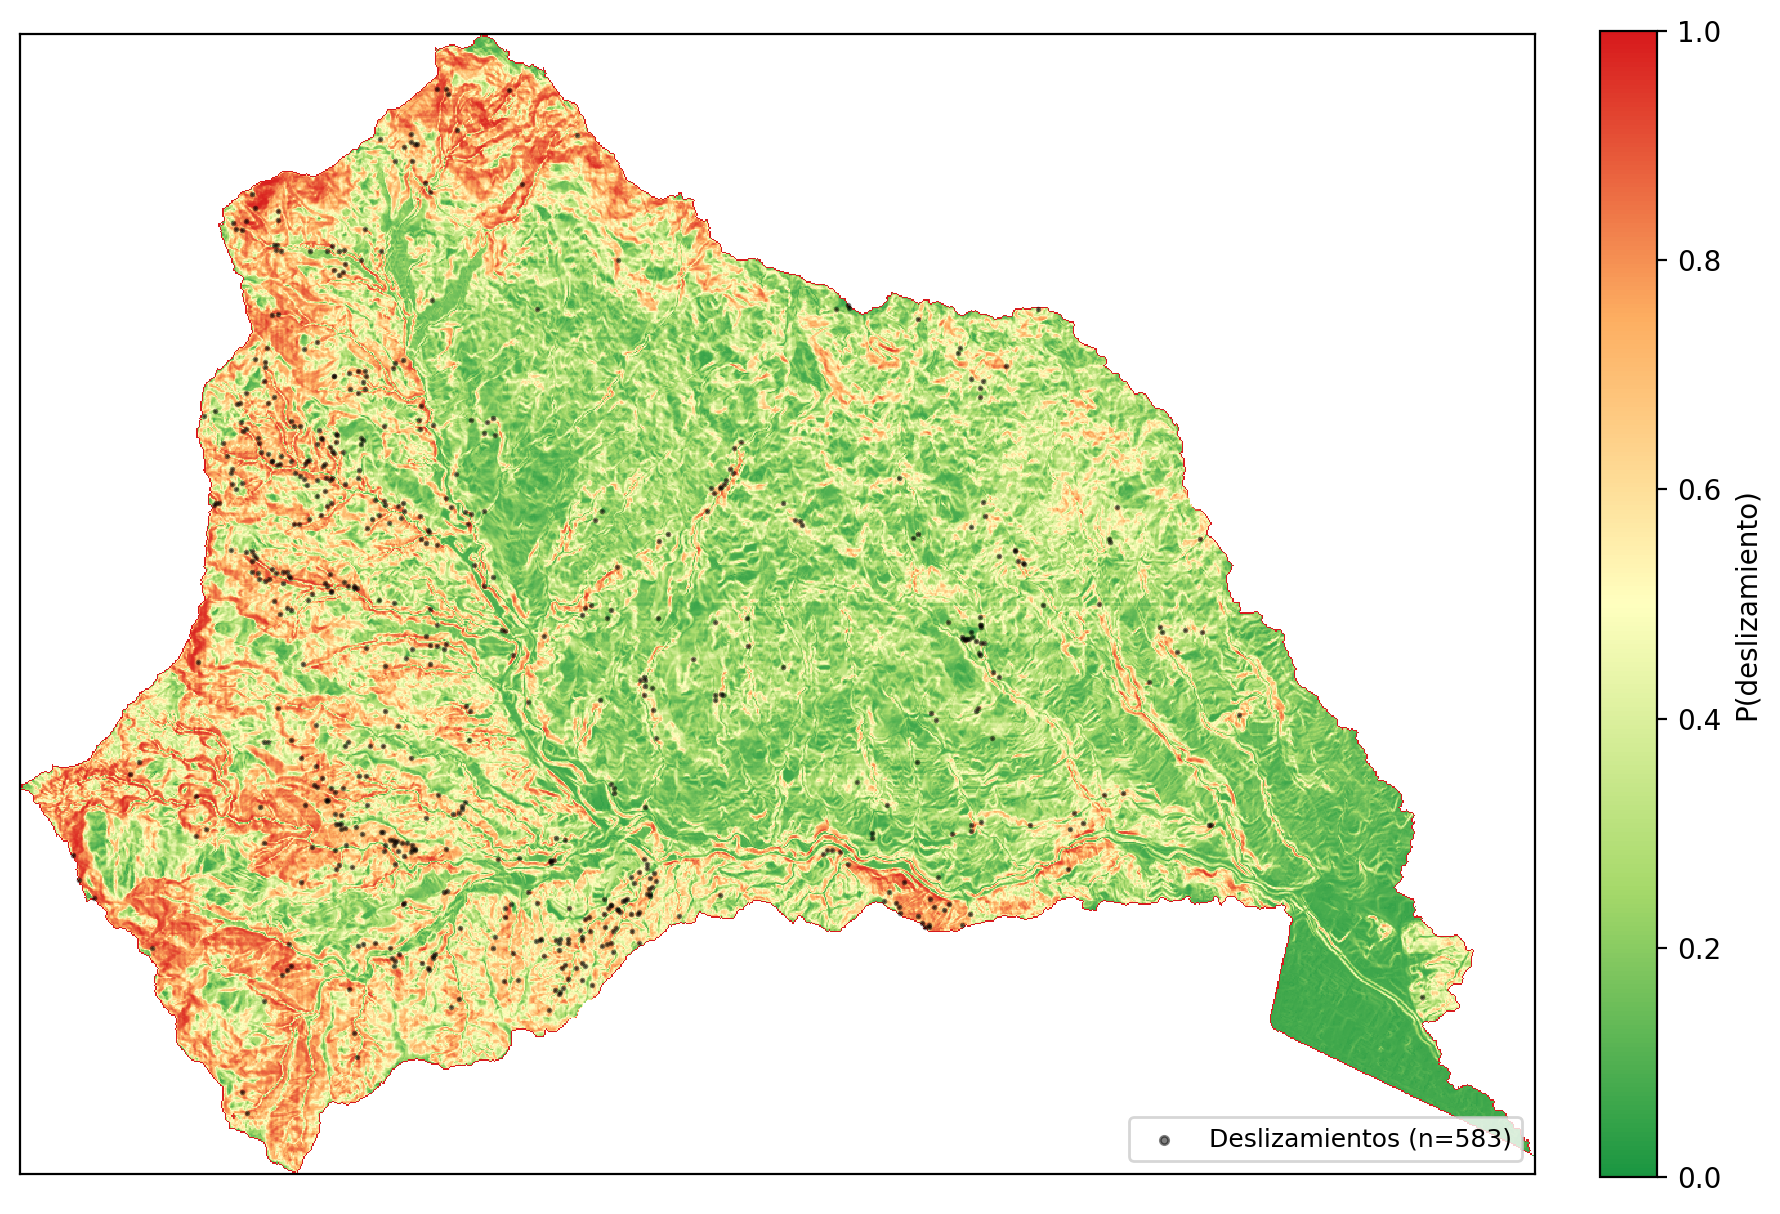
\includegraphics[width=0.65\textwidth]{Fig3_LR_susceptibility.png}
    \caption{Mapa de susceptibilidad por movimientos en masa de la regresión logística para la cuenca La Iguana. Escala de color: verde (Muy Baja, $P < 0{,}2$) a rojo oscuro (Muy Alta, $P > 0{,}8$). Los puntos negros indican las 583 ubicaciones de deslizamientos mapeados.}
    \label{fig:mapa_rl}
\end{figure}

\subsection{Distribución de clases de susceptibilidad}

La Figura~\ref{fig:clases} muestra la fracción del área en cada clase de susceptibilidad para el modelo RL. Aproximadamente el 36{,}8\% de la cuenca cae en las clases Alta o Muy Alta, el 26{,}3\% en la clase Moderada y el 36{,}9\% en las clases Baja o Muy Baja. Esta distribución es consistente con el carácter montañoso y empinado del terreno, donde una fracción significativa de las laderas supera el umbral morfológico de susceptibilidad moderada ($P > 0{,}4$).

\begin{figure}[H]
    \centering
    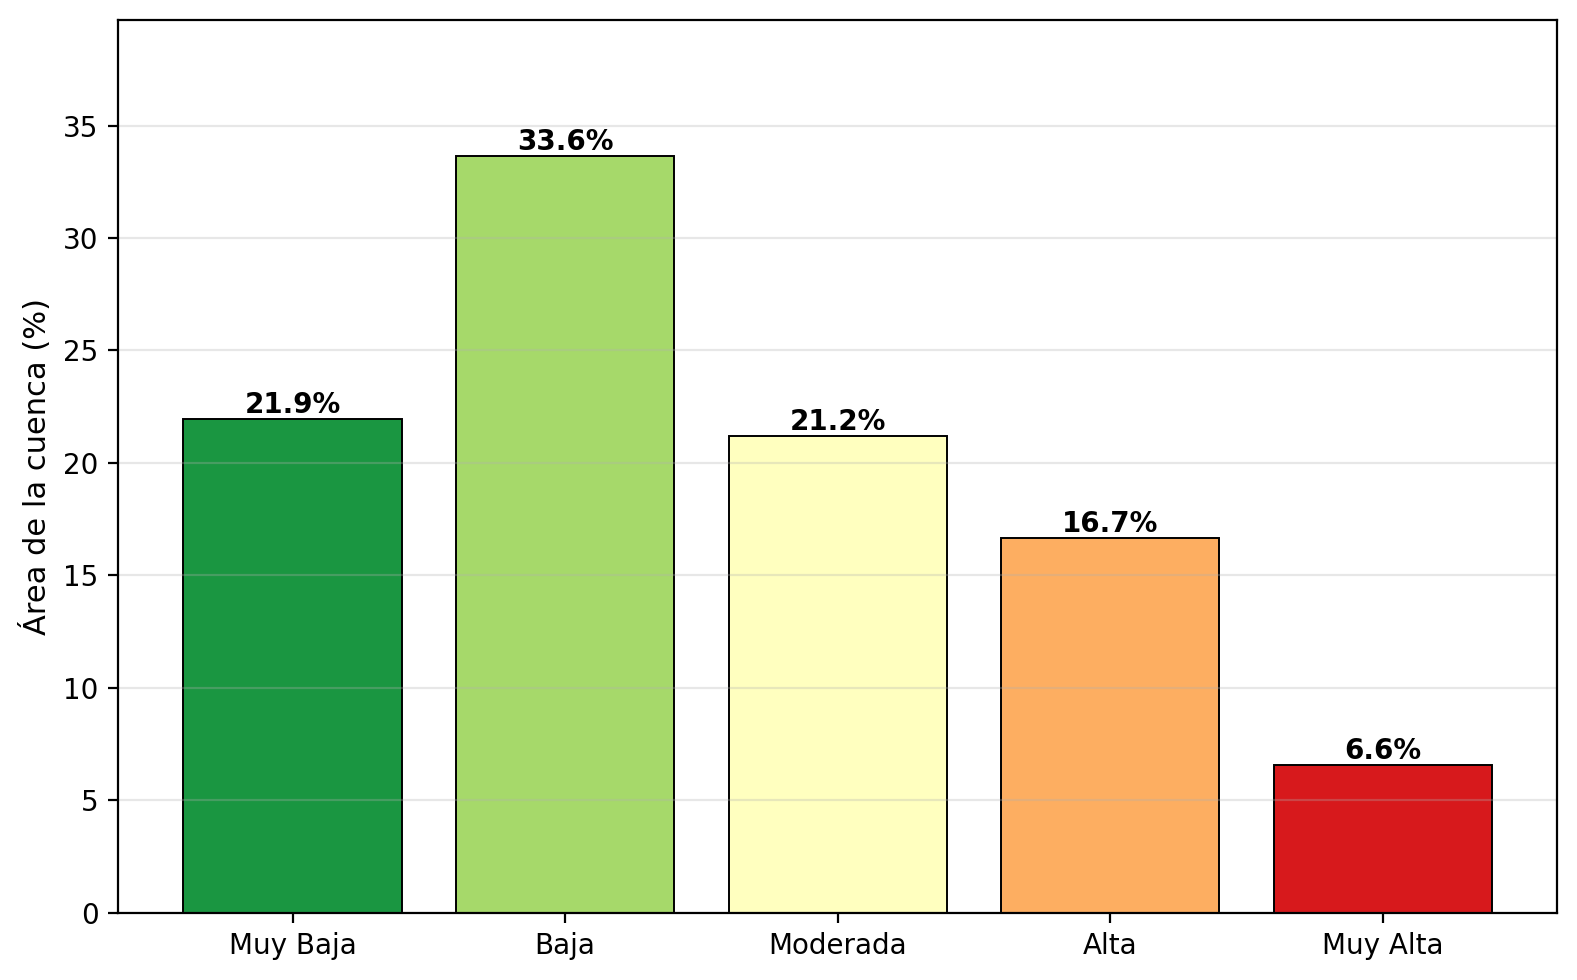
\includegraphics[width=0.65\textwidth]{Fig5_susceptibility_classes.png}
    \caption{Distribución del área de la cuenca La Iguana por clase de susceptibilidad según la regresión logística. Las clases se definen por intervalos de probabilidad iguales: Muy Baja $[0; 0{,}2)$, Baja $[0{,}2; 0{,}4)$, Moderada $[0{,}4; 0{,}6)$, Alta $[0{,}6; 0{,}8)$ y Muy Alta $[0{,}8; 1]$.}
    \label{fig:clases}
\end{figure}

\subsection{Modelo de proceso gaussiano}

La media posterior del PG (Fig.~\ref{fig:mapa_pg}a) reproduce estrechamente el patrón espacial de la superficie de susceptibilidad RL, como se esperaba dado que el PG es entrenado sobre las predicciones RL en las ubicaciones de deslizamientos. El núcleo de Matérn-$\nicefrac{3}{2}$ optimizado con longitud de escala $\hat{l} = 10{,}0$ en el espacio de covariables estandarizado indica que la función de susceptibilidad varía a escalas comparables al rango completo de covariables —una longitud de escala relativamente larga que sugiere una relación que varía suavemente—. La varianza de ruido optimizada casi nula ($\hat{\sigma}_n^2 \approx 10^{-4}$) indica que las probabilidades predichas por la RL en las ubicaciones de entrenamiento son internamente consistentes y contienen dispersión irreducible mínima.

El mapa de incertidumbre del PG (Fig.~\ref{fig:mapa_pg}b) es el valor añadido principal del enfoque de PG. Las desviaciones estándar posteriores ($\sigma$) son más bajas cerca de las zonas con densa cobertura de datos de entrenamiento en el espacio de covariables (es decir, cerca del clúster de deslizamientos en el espacio de pendiente alta / ITH moderado) y más altas en los extremos de la distribución de covariables —celdas planas del fondo del valle y laderas coluviales extremadamente empinadas en la periferia de la distribución de entrenamiento—. Esta estructura refleja la propiedad fundamental del PG de incrementar la incertidumbre en regiones extrapoladas, proporcionando orientación espacial sobre dónde los levantamientos de campo adicionales reducirían más efectivamente la varianza de la predicción.

\begin{figure}[H]
    \centering
    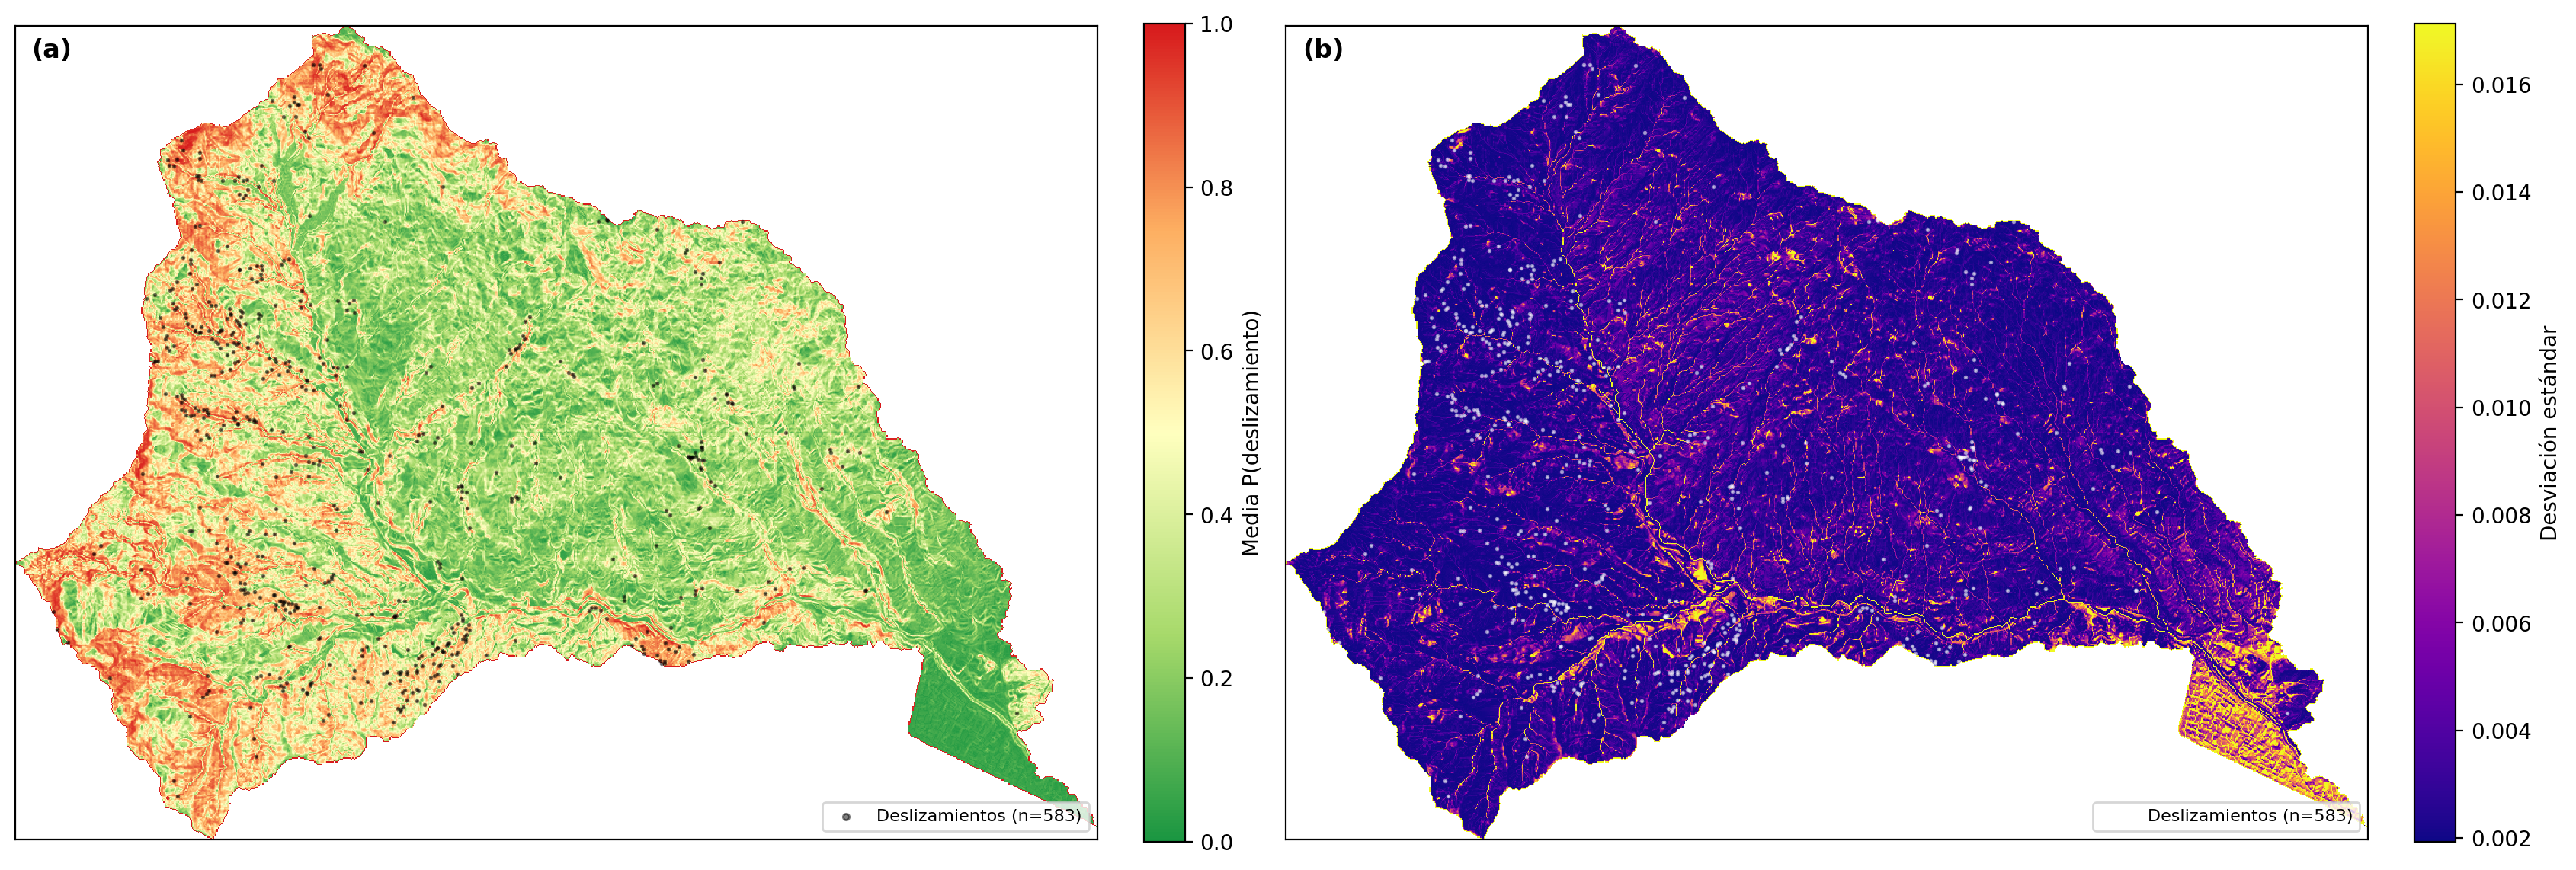
\includegraphics[width=\textwidth]{Fig4_GP_susceptibility_mean_std.png}
    \caption{Mapas del Proceso Gaussiano para la cuenca La Iguana. (a) Media posterior de la probabilidad predicha $\mu(\mathbf{x})$; los puntos negros indican las 583 ubicaciones de deslizamientos. (b) Desviación estándar posterior $\sigma(\mathbf{x})$, que cuantifica la incertidumbre de la predicción celda por celda; los puntos blancos indican las ubicaciones de deslizamientos. Valores altos de $\sigma$ señalan zonas donde el modelo está pobremente restringido por los datos de entrenamiento.}
    \label{fig:mapa_pg}
\end{figure}

\subsection{Análisis de la desviación estándar del proceso gaussiano}
\label{sec:analisis_std}

La Figura~\ref{fig:std_analisis} sintetiza el análisis de la distribución de la desviación estándar posterior $\sigma(\mathbf{x})$ a través de cuatro paneles complementarios: histograma de densidad, diagramas de caja por clase de susceptibilidad y diagramas de dispersión frente a cada covariable morfométrica.

\subsubsection{Distribución de la desviación estándar}

La distribución de $\sigma$ sobre la cuadrícula completa de la cuenca (Fig.~\ref{fig:std_analisis}a) es fuertemente asimétrica hacia la derecha, con una mediana de $0{,}0026$ y una media de $0{,}0041$, lo que indica que la mayor parte de la cuenca está bien restringida por los datos de entrenamiento. El percentil 95 es $0{,}011$ y el máximo absoluto alcanza $0{,}093$, correspondiendo este extremo a celdas en el fondo del valle y en el sector alto de la cuenca donde la densidad de deslizamientos en el espacio de covariables es mínima. La distribución de $\sigma$ en las ubicaciones de deslizamientos es notablemente más estrecha y desplazada hacia valores bajos respecto a la distribución de la cuenca completa (media en deslizamientos $\approx 0{,}0028$), lo cual es esperable: las ubicaciones de entrenamiento son precisamente las zonas del espacio de covariables mejor muestreadas por el PG.

\subsubsection{Desviación estándar por clase de susceptibilidad}

Los diagramas de caja (Fig.~\ref{fig:std_analisis}b) muestran una relación no monótona entre la clase de susceptibilidad y la incertidumbre. La clase Muy Alta ($P > 0{,}8$) exhibe una mediana de $\sigma$ baja y una caja compacta, lo que refleja que las celdas con pendientes muy pronunciadas —que dominan esta clase— corresponden a la región del espacio de covariables más densamente cubierta por los puntos de entrenamiento. La clase Muy Baja ($P < 0{,}2$), que agrupa las zonas de fondo de valle con pendientes bajas y alto ITH, presenta la mayor dispersión de $\sigma$ y la cola más larga, evidenciando que el PG extrapola con mayor incertidumbre hacia esta región donde los deslizamientos son escasos como datos de entrenamiento. Las clases intermedias (Baja y Moderada) muestran valores de $\sigma$ intermedios con mayor variabilidad, consistente con el hecho de que estas zonas transicionales ocupan regiones de covariable moderadamente alejadas del núcleo de entrenamiento.

\subsubsection{Relación entre covariables y desviación estándar}

Los diagramas de dispersión con la mediana por intervalo (Fig.~\ref{fig:std_analisis}c--e) y las correlaciones de rango de Spearman ($\rho$) revelan relaciones sistemáticas entre las covariables morfométricas y la incertidumbre del PG:

\begin{itemize}
    \item \textbf{Pendiente vs.\ $\sigma$} ($\rho = -0{,}619$, $p < 10^{-10}$): La correlación negativa fuerte indica que la incertidumbre disminuye sistemáticamente a medida que aumenta la pendiente. Esto es coherente con la distribución de los datos de entrenamiento: los 583 deslizamientos están concentrados en laderas de pendiente media-alta (20°--50°), de modo que el PG interpola con alta confianza en esta región pero extrapola con mayor incertidumbre hacia pendientes muy bajas ($< 10°$) donde los eventos de entrenamiento son escasos.

    \item \textbf{Aspecto vs.\ $\sigma$} ($\rho = +0{,}156$, $p < 10^{-10}$): La correlación positiva débil sugiere que las laderas con aspecto entre 180° y 360° (orientadas al S-O) tienden a presentar una incertidumbre ligeramente mayor. Este efecto secundario puede relacionarse con la distribución asimétrica del inventario, donde algunas orientaciones están subrepresentadas en los datos de entrenamiento.

    \item \textbf{ITH vs.\ $\sigma$} ($\rho = +0{,}665$, $p < 10^{-10}$): La correlación positiva fuerte con el ITH es el resultado más relevante: las celdas con valores altos de ITH (zonas convergentes, fondos de valle, canales) acumulan la mayor incertidumbre predictiva. Dado que los deslizamientos de tipo flujo son menos frecuentes en el inventario que los deslizamientos traslacionales de ladera, la región de alto ITH está pobremente representada en el conjunto de entrenamiento. Esto implica que, si bien el modelo asigna probabilidades bajas a estas zonas (consistente con el coeficiente negativo de la RL), la confianza en esa estimación es reducida. Este hallazgo tiene implicaciones directas para la gestión del riesgo: las zonas de canal y fondo de valle con alto ITH requieren validación de campo adicional antes de poder descartar su susceptibilidad con certeza.
\end{itemize}

\begin{figure}[H]
    \centering
    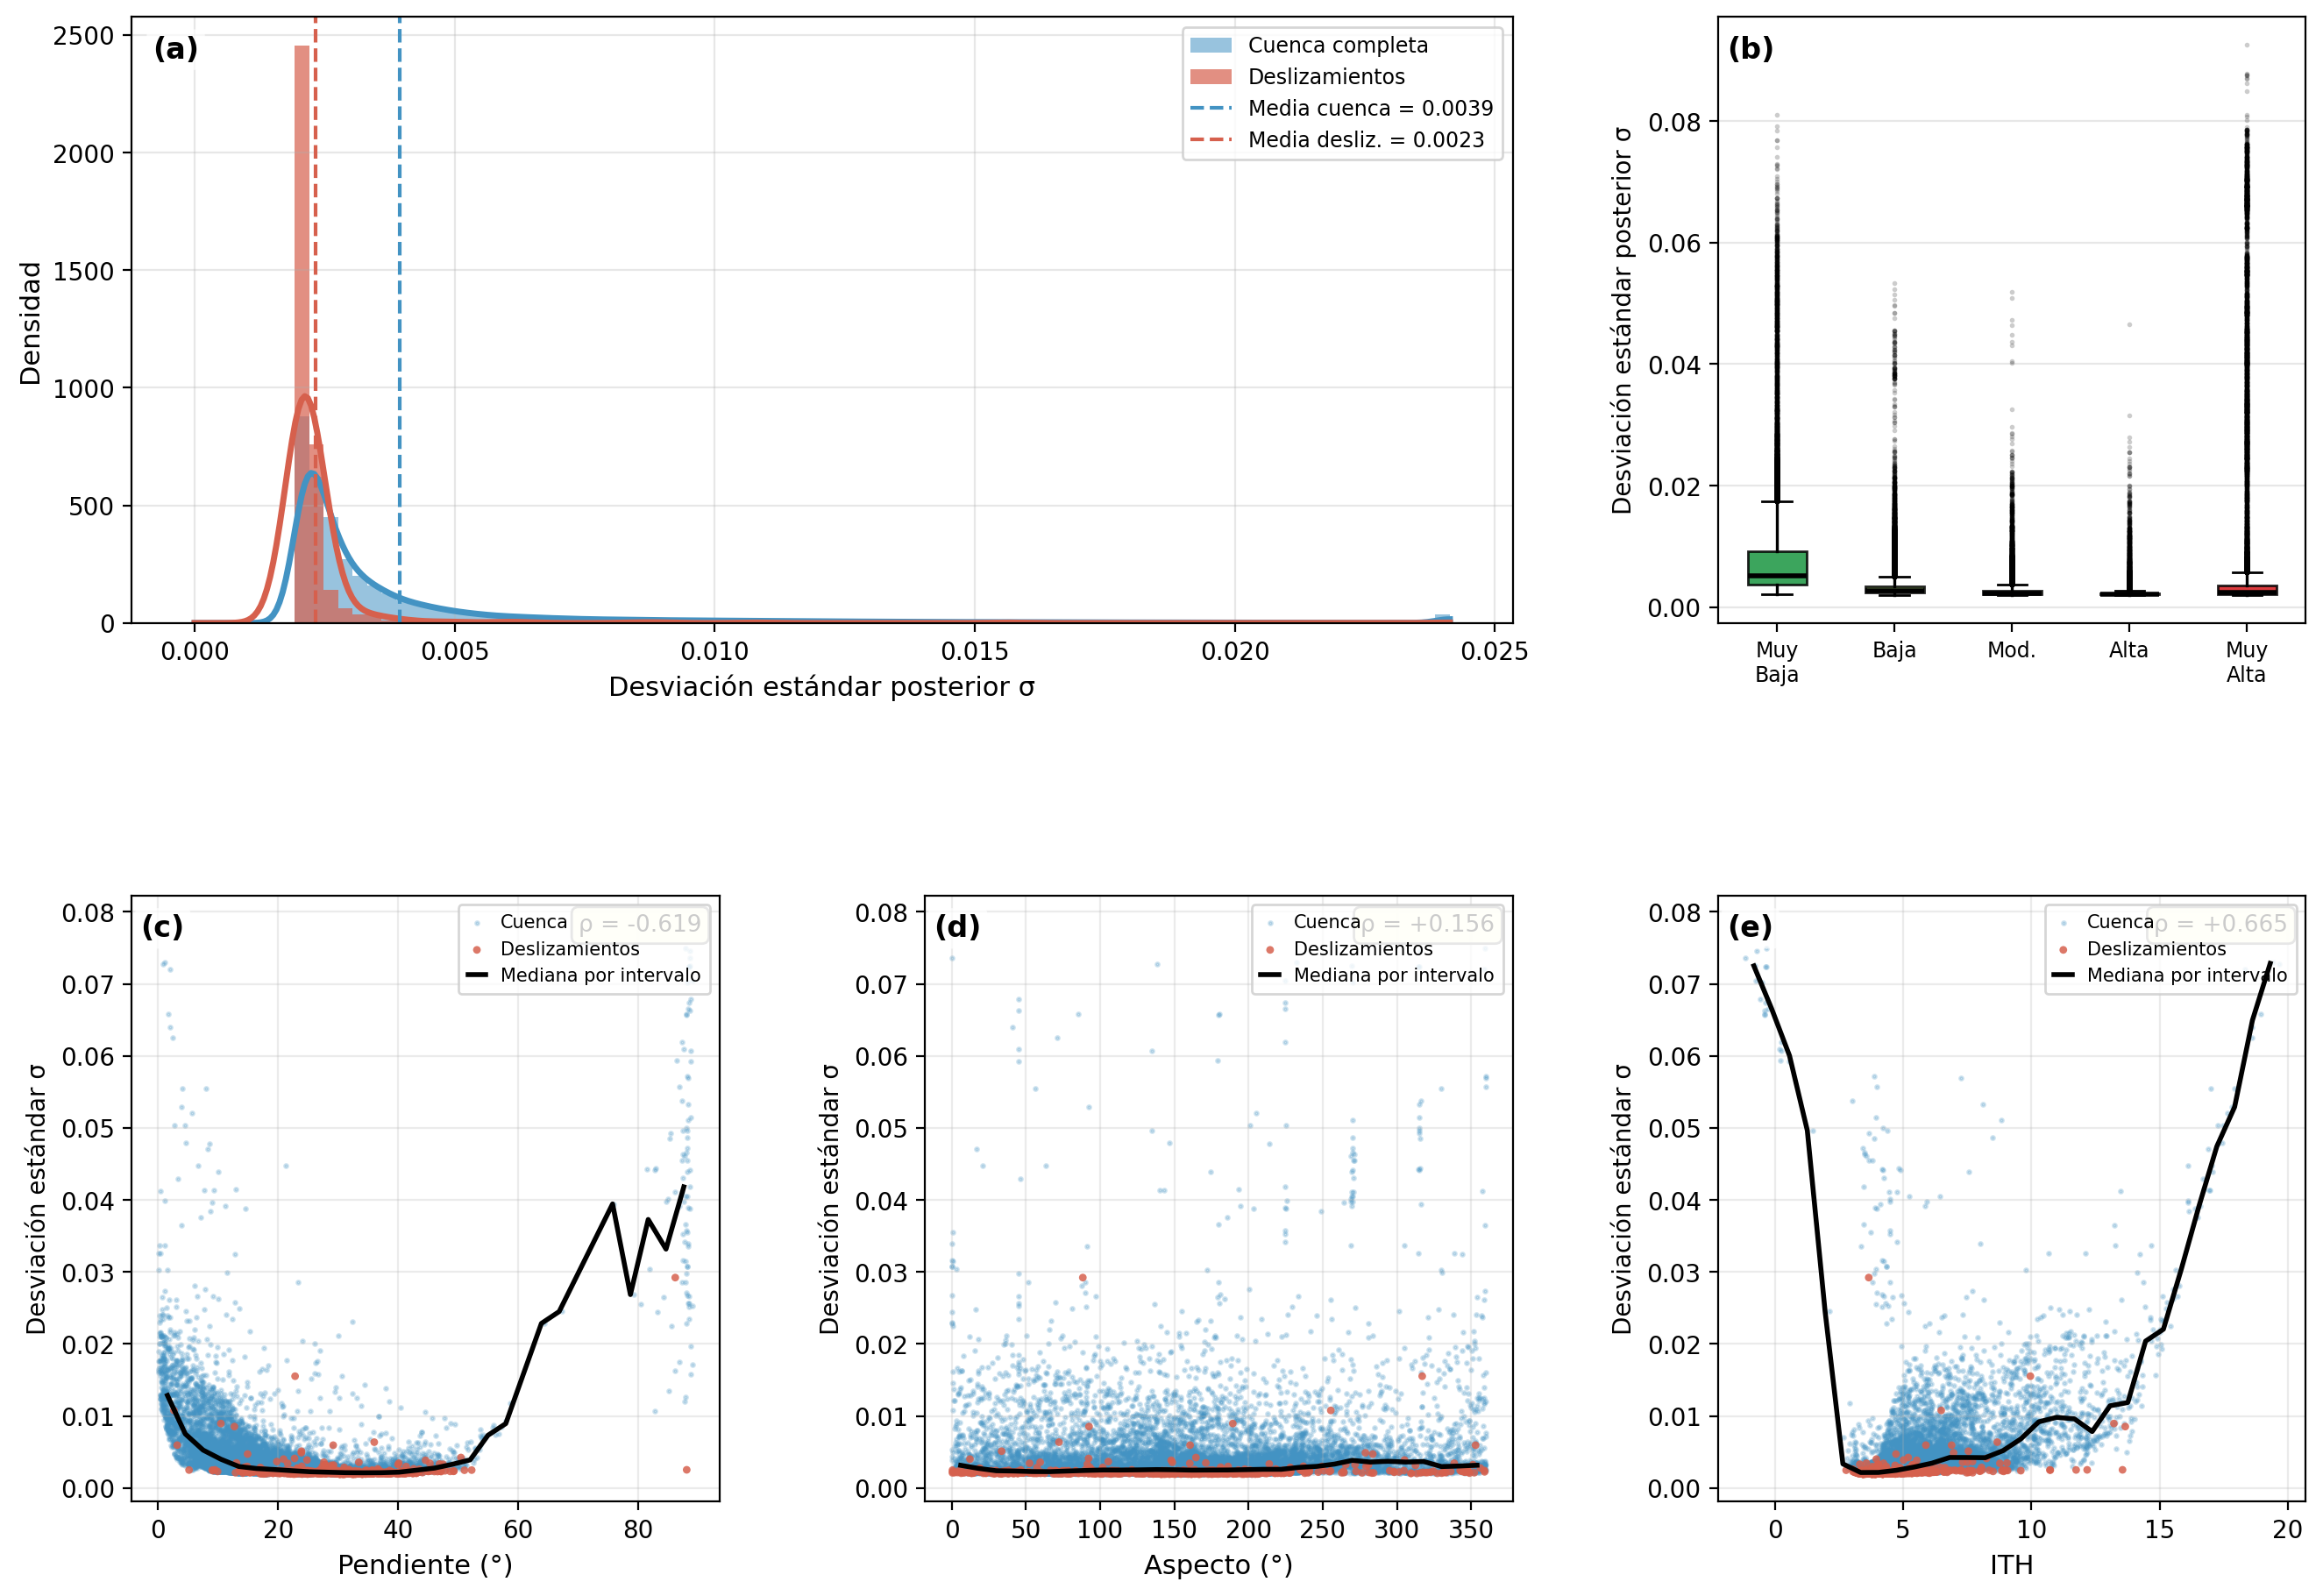
\includegraphics[width=\textwidth]{Fig7_GP_std_analysis.png}
    \caption{Análisis de la desviación estándar posterior $\sigma(\mathbf{x})$ del Proceso Gaussiano sobre la cuenca La Iguana. (a) Histograma de densidad y estimación por núcleo gaussiano (KDE) de $\sigma$ para la cuenca completa (azul) y para las ubicaciones de deslizamientos (rojo); las líneas discontinuas indican las medias respectivas. (b) Diagramas de caja de $\sigma$ estratificados por clase de susceptibilidad de la regresión logística; los colores de las cajas corresponden a la escala de susceptibilidad (verde = Muy Baja, rojo = Muy Alta). (c)--(e) Diagramas de dispersión de $\sigma$ frente a pendiente (c), aspecto (d) e ITH (e); puntos azules = muestra aleatoria de celdas de la cuenca; puntos rojos = ubicaciones de deslizamientos; línea negra = mediana de $\sigma$ por intervalo de la covariable; $\rho$ = correlación de Spearman (todos los valores son estadísticamente significativos, $p < 10^{-10}$).}
    \label{fig:std_analisis}
\end{figure}

\subsection{Métricas de desempeño}

La Tabla~\ref{tab:metricas} resume las métricas de discriminación y calibración para ambos modelos evaluados sobre la cuadrícula completa de la cuenca. A nivel de celda, la precisión y la puntuación F1 en el umbral de 0{,}5 son extremadamente bajas debido al desequilibrio de clases natural ($\approx 0{,}11\%$ de tasa positiva); la AUC y la AP son por tanto los indicadores de discriminación primarios.

\begin{table}[H]
    \centering
    \caption{Métricas de desempeño de la regresión logística y el proceso gaussiano evaluadas sobre la cuadrícula completa de la cuenca ($n = 521{,}586$ celdas; 583 positivos). AP = Precisión Promedio. Umbral de clasificación = 0{,}5.}
    \label{tab:metricas}
    \begin{tabular}{lccccccc}
        \toprule
        Modelo & AUC-ROC & AP & Exactitud & Precisión & Exhaustividad & F1 & Brier \\
        \midrule
        Regresión logística & 0{,}765 & 0{,}003 & 0{,}671 & 0{,}003 & 0{,}762 & 0{,}005 & 0{,}218 \\
        Proceso gaussiano   & 0{,}765 & 0{,}003 & 0{,}671 & 0{,}003 & 0{,}762 & 0{,}005 & 0{,}218 \\
        \bottomrule
    \end{tabular}
\end{table}

Las métricas de discriminación son prácticamente idénticas para ambos modelos. Esto es esperado por diseño: el PG fue entrenado para aproximar la función RL en el espacio de covariables, de modo que su desempeño discriminativo no puede superar al de la RL. La diferencia fundamental entre los dos enfoques no reside en las métricas de discriminación sino en la capacidad del PG de cuantificar explícitamente la incertidumbre de la predicción —información que la RL no proporciona—.

% =========================================================
\section{Discusión}
\label{sec:discusion}

\subsection{Desempeño predictivo de las covariables topográficas}

El modelo RL alcanza una AUC validada de $0{,}788 \pm 0{,}025$, dentro del rango reportado para modelos RL con solo topografía en cuencas andinas tropicales comparables \citep{Pradhan2010, Chen2017}. El papel dominante de la pendiente ($\hat{\beta}_\mathrm{pendiente} = +1{,}193$) confirma que las fuerzas motrices gravitacionales siguen siendo el control de primer orden sobre la iniciación de movimientos en masa superficiales, consistente con la teoría de estabilidad de pendiente infinita \citep{Varnes1978}. La contribución limitada del ITH a la discriminación del modelo —a pesar de su relevancia física establecida para la dinámica de la presión de poros— probablemente refleja limitaciones del MDE de 10 m para resolver las hondonadas microtopográficas donde ocurre la saturación transitoria real, así como el supuesto de estado estacionario subyacente a la formulación del ITH, que puede representar mal los patrones de saturación episódicos impulsados por la lluvia que desencadenan deslizamientos en esta región \citep{Aristizabal2023}.

Los valores absolutos de AUC moderados, aunque aceptables para un modelo de solo topografía, destacan el conocido desafío de lograr alta discriminación con atributos del terreno en pequeñas cuencas urbanas empinadas donde la heterogeneidad litológica, el espesor del suelo, los patrones de uso del suelo y la humedad antecedente también ejercen controles significativos \citep{Reichenbach2018}. El trabajo futuro debería incorporar estimaciones de profundidad del suelo, mapas geológicos a escala 1:10.000 e índices de vegetación derivados de satélites para mejorar la discriminación.

\subsection{Interpretación física de la estructura de incertidumbre del proceso gaussiano}

El análisis de la desviación estándar posterior $\sigma(\mathbf{x})$ revela una estructura de incertidumbre con claro fundamento físico-estadístico. La fuerte correlación negativa entre pendiente y $\sigma$ ($\rho = -0{,}619$) y la correlación positiva fuerte entre ITH y $\sigma$ ($\rho = +0{,}665$) son interpretables en términos de la distribución de los datos de entrenamiento en el espacio de covariables: el PG presenta baja incertidumbre precisamente donde los deslizamientos del inventario están concentrados (laderas empinadas de pendiente 20°--50°), y alta incertidumbre donde los deslizamientos son escasos como observaciones de entrenamiento (zonas planas de alto ITH). Este comportamiento es una consecuencia directa de la propiedad fundamental de los procesos gaussianos de incrementar la varianza posterior a medida que las predicciones se alejan de los puntos de entrenamiento en el espacio de covariables \citep{Rasmussen2006}.

Desde la perspectiva de la gestión del riesgo, estos resultados tienen una implicación práctica concreta: las zonas de fondo de valle y canales con alto ITH —que el modelo RL clasifica como de baja susceptibilidad por la relación negativa del coeficiente del ITH— son precisamente las zonas donde esa estimación es más incierta. La incertidumbre alta en estas zonas no significa necesariamente que el riesgo sea elevado, pero sí que el modelo no tiene suficiente información para afirmar con confianza que el riesgo es bajo. Esta distinción es crítica en planificación territorial: una zona de susceptibilidad baja pero con alta $\sigma$ debe tratarse con más cautela que una zona de susceptibilidad igualmente baja pero con $\sigma$ reducido, y debería ser priorizada para validación en campo. El enfoque de RL convencional, al producir solo una estimación puntual, es incapaz de hacer esta diferenciación.

\subsection{El proceso gaussiano como complemento de la regresión logística}

La distinción más importante entre el PG y la RL no es el desempeño de discriminación —que es similar para ambos— sino la \emph{naturaleza de la salida}. El PG proporciona una distribución posterior completa sobre la función de susceptibilidad, expresada como media y desviación estándar en cada celda de la cuadrícula. Esta cuantificación de la incertidumbre está ausente en la salida estándar de la RL y tiene un valor operativo significativo:

\begin{enumerate}
    \item \textbf{Identificación de brechas de datos}: Las zonas con $\sigma(\mathbf{x})$ elevado revelan regiones de covariables pobremente restringidas por los datos de entrenamiento, orientando campañas de campo focalizadas para completar el inventario.
    \item \textbf{Comunicación conservadora del riesgo}: En zonas de alta incertidumbre, los gestores de riesgo pueden optar por adoptar un límite superior precautorio de la susceptibilidad (p. ej., $\mu + k\sigma$ para algún $k > 0$) en lugar de confiar en la estimación puntual.
    \item \textbf{Análisis probabilístico de umbrales}: A diferencia de una puntuación única de susceptibilidad, la posterior del PG permite enunciados de probabilidad explícitos de la forma $P(\hat{p} > p_{\mathrm{umbral}})$ para cualquier umbral $p_{\mathrm{umbral}}$, lo que es útil para el diseño de ordenanzas de zonificación.
\end{enumerate}

La AUC casi idéntica entre RL y PG sobre la cuadrícula completa refleja la elección de diseño de usar las predicciones de la RL como objetivos del PG: por construcción, el PG aproxima la función RL en el espacio de covariables, de modo que su desempeño discriminativo esperado no puede superar al de la RL. Una formulación alternativa del PG —usando las etiquetas binarias $\{0,1\}$ como objetivos (es decir, clasificación por PG mediante propagación de expectativas)— sería más independiente de la RL y potencialmente capaz de superarla, al costo de una inferencia aproximada más compleja. Esto permanece como una vía de desarrollo futuro.

\subsection{Escalabilidad computacional}

La principal limitación práctica del enfoque de PG es el costo computacional. Con $n$ puntos de entrenamiento, la inferencia exacta requiere tiempo $\mathcal{O}(n^3)$ y memoria $\mathcal{O}(n^2)$, haciendo el PG exacto inviable para $n \gtrsim 10^4$. Se abordó esto submuestreando a 400 puntos, lo que introduce un pequeño error de aproximación relativo al uso de las 580 celdas únicas de deslizamientos. Las aproximaciones de PG disperso —como los métodos de puntos inductores (FITC, VFE) \citep{Rasmussen2006} o el PG variacional estocástico \citep{Lombardo2020}— podrían recuperar la posterior de datos completos a una fracción del costo y deberían explorarse en trabajos futuros, particularmente para inventarios más grandes o MDE de mayor resolución.

\subsection{Limitaciones y direcciones futuras}

Varias limitaciones de este estudio merecen reconocimiento explícito:

\begin{itemize}
    \item \textbf{Completitud del inventario}: El inventario captura principalmente eventos del período 2010--2023 identificados mediante teledetección y levantamientos de campo; los eventos más antiguos y de menor tamaño pueden estar sistemáticamente subrepresentados, sesgando potencialmente los datos de entrenamiento hacia regiones específicas de covariables.
    \item \textbf{Estacionariedad temporal}: Ambos modelos asumen que la relación covariable-deslizamiento es estacionaria en el tiempo, mientras que las proyecciones de cambio climático sugieren una intensificación de la lluvia extrema en los Andes colombianos \citep{Aristizabal2023}, lo que podría desplazar el panorama de susceptibilidad.
    \item \textbf{Controles no topográficos}: El uso del suelo, la carga antrópica y la infraestructura modulan la susceptibilidad a la falla en esta cuenca periurbana, pero actualmente no están incluidos en el modelo.
    \item \textbf{Formulación por proceso de puntos}: Tanto la RL como el PG son aquí tratados como modelos a nivel de celda, ignorando la agrupación espacial de deslizamientos y la estructura de dependencia de fallas vecinas. Las extensiones por proceso de puntos \citep{Lombardo2019} ofrecen un tratamiento más fundamentado de la dependencia entre eventos.
\end{itemize}

% =========================================================
\section{Conclusiones}
\label{sec:conclusiones}

Este estudio presentó y evaluó un marco probabilístico de dos etapas para la cartografía de susceptibilidad por movimientos en masa en la cuenca La Iguana (Medellín, Colombia), combinando regresión logística (RL) y proceso gaussiano de regresión (PGR) con covariables topográficas (pendiente, aspecto, ITH) derivadas de un MDE de 10 m.

Las principales conclusiones son:

\begin{enumerate}
    \item Un modelo de regresión logística con predictores puramente topográficos alcanza una AUC validada con cinco pliegues de $0{,}788 \pm 0{,}025$ en esta cuenca urbana andina de alta pendiente, confirmando que la morfometría del terreno por sí sola proporciona una señal de susceptibilidad de primer orden útil. La pendiente es el predictor dominante, con un coeficiente estandarizado de $+1{,}193$.

    \item El proceso gaussiano condicionado sobre las predicciones de la RL en las ubicaciones de deslizamientos reproduce el desempeño discriminativo del modelo RL (AUC = $0{,}765$, índice de Brier = $0{,}218$) mientras que adicionalmente proporciona mapas de incertidumbre espacialmente explícitos —una característica no disponible en la RL estándar—. El núcleo de Matérn-$\nicefrac{3}{2}$ optimizado indica una estructura de covarianza suave y de larga longitud de escala en el espacio de covariables.

    \item El análisis de la desviación estándar posterior del PG revela una estructura de incertidumbre estadística y físicamente coherente: $\sigma$ correlaciona negativamente con la pendiente ($\rho = -0{,}619$) y positivamente con el ITH ($\rho = +0{,}665$), de modo que la mayor incertidumbre se concentra en las zonas de fondo de valle y canales de alto ITH —regiones pobremente representadas en el inventario de entrenamiento—. Este resultado orienta de forma objetiva la priorización de campañas de validación en campo y diferencia zonas de susceptibilidad baja pero incierta de zonas de susceptibilidad baja y bien restringida, distinción imposible de hacer con la RL estándar.

    \item Aproximadamente el 37\% de la cuenca La Iguana se clasifica como susceptibilidad Alta o Muy Alta bajo el modelo RL, predominantemente en flancos de canales empinados y hondonadas convergentes entre 1700 y 2400 m de elevación —zonas que deberían recibir atención prioritaria en los planes de gestión del riesgo por movimientos en masa del Área Metropolitana del Valle de Aburrá—.

    \item El marco de PG es computacionalmente viable para cientos de puntos de entrenamiento en una estación de trabajo estándar, y su integración con los flujos de trabajo RL existentes requiere un esfuerzo de implementación adicional mínimo, lo que lo convierte en una herramienta práctica para la cartografía operacional de susceptibilidad.
\end{enumerate}

El trabajo futuro debería ampliar el conjunto de covariables para incluir información geológica, edafológica y de uso del suelo; adoptar aproximaciones de PG disperso para escalar a inventarios más grandes; y explorar formulaciones de clasificación por PG que no dependan de los objetivos predichos por la RL, permitiendo una cuantificación de la incertidumbre completamente independiente.

% =========================================================
\section*{Disponibilidad de datos}

El MDE y el límite de la cuenca están disponibles a través del Área Metropolitana del Valle de Aburrá (AMVA). El inventario de movimientos en masa hace parte de un catálogo regional en curso mantenido por la Universidad Nacional de Colombia, Sede Medellín. El código de análisis completo y el cuaderno Jupyter están disponibles como material suplementario de este manuscrito.

\section*{Agradecimientos}

Los autores reconocen al Área Metropolitana del Valle de Aburrá (AMVA) y al Sistema de Alerta Temprana de Medellín y el Valle de Aburrá (SIATA) por proporcionar datos geoespaciales. Esta investigación fue parcialmente apoyada por la Universidad Nacional de Colombia, Sede Medellín.

\section*{Conflicto de intereses}

Los autores declaran no tener conflicto de intereses.

% =========================================================
\bibliographystyle{apalike}
\bibliography{referencias}

\end{document}
